\documentclass[11pt]{article}
\usepackage[margin=18mm,headheight=22pt]{geometry}
\usepackage{amsmath}
\usepackage{fontspec}
\usepackage{unicode-math}
\setmainfont{NewCM10}[Extension=.otf,UprightFont=*-Book,BoldFont=*-Bold,ItalicFont=*-BookItalic,BoldItalicFont=*-BoldItalic]
\setsansfont{NewCMSans10}[Extension=.otf,UprightFont=*-Book,BoldFont=*-Bold,ItalicFont=*-BookOblique,BoldItalicFont=*-BoldOblique]
\setmathfont{NewCMMath-Book.otf}
\usepackage{xcolor}
\definecolor{FAUblue}{HTML}{04316A}
\definecolor{Paperblue}{HTML}{EEF2F7}
\definecolor{EEIgold}{HTML}{CC9C42}
\usepackage{etoolbox,enumitem,booktabs,tabularx,array,needspace,microtype}
\usepackage[most]{tcolorbox}
\usepackage{titlesec,fancyhdr}
\usepackage[hidelinks]{hyperref}
\usepackage{draftwatermark}
\SetWatermarkText{Made by Thanate Amornjiraporn (Focus)}
\SetWatermarkColor{black!7}\SetWatermarkFontSize{30pt}\SetWatermarkAngle{45}
\setlength{\parindent}{0pt}
\setlength{\parskip}{5pt}
\setlist{itemsep=2pt,topsep=3pt,leftmargin=1.6em,beginpenalty=10000,endpenalty=10000}
\raggedbottom
\clubpenalty=10000 \widowpenalty=10000 \displaywidowpenalty=10000 \interlinepenalty=10000
\setcounter{secnumdepth}{0}
\setcounter{tocdepth}{1}
\pagestyle{fancy}\fancyhf{}
\fancyhead[L]{\small\sffamily\color{FAUblue} From Fundamentals to AI Apocalypse · EEI · Chapter 3}
\fancyhead[R]{\small\sffamily DC Networks}
\fancyfoot[C]{\small\thepage}
\titleformat{\section}{\Large\bfseries\sffamily\color{FAUblue}}{}{0pt}{}
\titleformat{\subsection}{\large\bfseries\sffamily\color{FAUblue}}{}{0pt}{}
\titlespacing*{\section}{0pt}{16pt}{6pt}
\preto\section{\Needspace{8\baselineskip}}
\preto\subsection{\Needspace{6\baselineskip}}
\newtcolorbox{equationcard}[1]{colback=Paperblue,colframe=Paperblue,boxrule=0pt,arc=0pt,left=10pt,right=10pt,top=6pt,bottom=6pt,title={#1},fonttitle=\small\bfseries\sffamily,coltitle=FAUblue,before skip=8pt,after skip=8pt}
\newtcolorbox{workedbox}[1]{colback=white,colframe=EEIgold,boxrule=0pt,leftrule=3pt,arc=0pt,left=10pt,top=4pt,bottom=4pt,title={#1},fonttitle=\small\bfseries\sffamily,coltitle=FAUblue,attach title to upper={\par},before skip=8pt,after skip=8pt}
\newtcolorbox{recallbox}[1]{colback=white,colframe=FAUblue,boxrule=0pt,leftrule=3pt,arc=0pt,left=10pt,top=4pt,bottom=4pt,title={#1},fonttitle=\small\bfseries\sffamily,coltitle=FAUblue,attach title to upper={\par},before skip=8pt,after skip=8pt}
\usepackage{environ}
\newsavebox\measurebox
% Typeset the section once invisibly to measure it; start a new page if it will not fit in what is left.
\makeatletter
\newif\ifkeep@measuring
\NewEnviron{keepsection}{%
  \ifkeep@measuring \BODY \else
    \edef\keep@sec{\the\value{section}}\edef\keep@sub{\the\value{subsection}}%
    \setbox\measurebox\vbox{\hsize\linewidth\keep@measuringtrue\def\Needspace##1{}\BODY}%
    \setcounter{section}{\keep@sec}\setcounter{subsection}{\keep@sub}%
    \dimen2=\ht\measurebox \advance\dimen2\dp\measurebox
    \dimen@=\textheight
    \ifdim\pagegoal<\maxdimen
      \dimen@=\pagegoal \advance\dimen@-\pagetotal
      \ifdim\dimen2>\dimen@ \clearpage \dimen@=\textheight \fi
    \fi
    % if it fits, nothing inside may force an early break
    \ifdim\dimen2>\dimen@ \BODY \else \begingroup\def\Needspace##1{}\BODY\endgroup \fi
  \fi}
\makeatother
\newtcolorbox{notebox}{colback=Paperblue,colframe=Paperblue,boxrule=0pt,arc=0pt,left=8pt,right=8pt,top=4pt,bottom=4pt,before skip=6pt,after skip=6pt}
\newtcolorbox{plainbox}{colback=white,colframe=FAUblue,boxrule=0pt,leftrule=3pt,arc=0pt,left=10pt,right=8pt,top=4pt,bottom=4pt,before skip=6pt,after skip=8pt}
\usetikzlibrary{arrows.meta}
\title{\sffamily\bfseries\color{FAUblue}DC Networks}
\author{Electrical Engineering I \ensuremath{\cdot} Module 92315 \ensuremath{\cdot} Chapter 3\\[2pt]\small From Fundamentals to AI Apocalypse · personal study guide}
\date{}
\begin{document}
\maketitle
\begingroup\footnotesize\setlength{\parskip}{0pt}\tableofcontents\endgroup
\clearpage

\Needspace{10\baselineskip}
{\large Chapters 1 and 2 described fields inside components; this chapter treats each component as a box with two terminals and a current–voltage rule. With sources, Kirchhoff’s two laws and a few reduction rules you can find every current and voltage in a resistor network, and judge how much power reaches a load.}


\begin{keepsection}
\Needspace{18\baselineskip}
\section{Start from memory}

\Needspace{15\baselineskip}
Try these before reading. Write an answer even if you are uncertain; the gap tells you what to look for.

\Needspace{12\baselineskip}
\begin{enumerate}
\item Two resistors of 6 Ω and 3 Ω are connected in series, then in parallel. What is the total resistance each time?
\item Why does a battery’s terminal voltage drop when it delivers a large current?
\item What do the voltages round any closed loop of a circuit add up to?
\item Three wires meet at a point. 2 A flows in on one and 0.5 A flows out on another. What flows on the third?
\item Which load resistance takes the most power from a source with internal resistance \textit{R}\textsubscript{i}?
\item A circuit has two sources. Can you find a current by switching on one source at a time?
\end{enumerate}

\nopagebreak[4]{\small\itshape Answers: see “Start from memory” under Answers at the end.}
\end{keepsection}

\begin{keepsection}
\Needspace{23\baselineskip}
\section{How to use this guide}

\Needspace{20\baselineskip}
Attempt each worked example before reading its steps. Then hide the guide and retrieve the method on a later day.

\Needspace{17\baselineskip}
\begin{enumerate}
\item \textbf{Day 0:} Do the cold start. Read §3.1–§3.3 and redraw one circuit of your own as a network graph with numbered nodes and branches.
\item \textbf{Day 1:} Study §3.4. Write Kirchhoff’s laws for the mesh and node figures without looking, then try the mixed-practice problems on §3.1–§3.4: 2, 3, 5, 7, 8, 10, 13, 15, 17, 20, 23 and 24.
\item \textbf{Day 3:} Study §3.5. Rebuild the divider and maximum-power derivations from a blank page, then solve the §3.5 problems 1, 6, 11, 12, 16, 19 and 22 without notes.
\item \textbf{About day 7:} Study §3.6. Run the seven node-voltage steps on the worked circuit from memory, then solve the §3.6 problems 4, 9, 14, 18 and 21. Finally shuffle all 24 and say, for each, which tool you would choose.
\item \textbf{About day 14:} Rebuild every derivation in “Derive it cold” and retry every question you marked. Tick the self-check only with evidence from unaided work.
\item \textbf{Before the exam:} Do both exam problems under the time limit, then review only the skills your evidence shows are weak.
\end{enumerate}
\end{keepsection}

\begin{keepsection}
\Needspace{25\baselineskip}
\section{How the chapter fits together}

\Needspace{22\baselineskip}
Every component is reduced to its terminal rule: a resistor obeys Ohm’s law, a source fixes a voltage or a current. Kirchhoff’s two laws then tie the components together. Everything else in the chapter is a shortcut built from those three ingredients, or, for larger networks, a systematic way to write them down.

\Needspace{11\baselineskip}
\subsection{Measured \ensuremath{\cdot} the parts}

\Needspace{8\baselineskip}
\begin{itemize}
\item \Needspace{4\baselineskip}
\textbf{Ohm’s law at the terminals} \hfill{\small\color{FAUblue}§3.1}

\Needspace{4\baselineskip}
U = RI, G = {\small\ensuremath{\dfrac{1}{\mathrm{R}}}}

Rests on: describing each resistor only by its terminal rule, with R \ensuremath{>} 0.
\item \Needspace{4\baselineskip}
\textbf{Ideal and real sources} \hfill{\small\color{FAUblue}§3.2}

\Needspace{4\baselineskip}
U = U\textsubscript{0} \ensuremath{-} IR\textsubscript{i}

Rests on: a fixed voltage or current, plus an internal resistance.
\item \Needspace{4\baselineskip}
\textbf{Nodes, branches, arrows} \hfill{\small\color{FAUblue}§3.3}

\Needspace{4\baselineskip}
load and generator convention

Rests on: drawing a reference arrow for every branch voltage and current.
\end{itemize}

\Needspace{11\baselineskip}
\subsection{Defined \ensuremath{\cdot} the connection rules}

\Needspace{8\baselineskip}
\begin{itemize}
\item \Needspace{4\baselineskip}
\textbf{Kirchhoff’s voltage law} \hfill{\small\color{FAUblue}§3.4}

\Needspace{4\baselineskip}
\ensuremath{\textstyle\sum} U = 0 round a mesh

Rests on: the closed line integral of the static field being zero.
\item \Needspace{4\baselineskip}
\textbf{Kirchhoff’s current law} \hfill{\small\color{FAUblue}§3.4}

\Needspace{4\baselineskip}
\ensuremath{\textstyle\sum} I = 0 at a node

Rests on: charge being conserved in stationary currents.
\item \Needspace{4\baselineskip}
\textbf{Source transformation} \hfill{\small\color{FAUblue}§3.2}

\Needspace{4\baselineskip}
U\textsubscript{0} = I\textsubscript{0}R\textsubscript{i}

Rests on: both models having the same open-circuit voltage and short-circuit current.
\end{itemize}

\Needspace{15\baselineskip}
\subsection{Derived \ensuremath{\cdot} tools you calculate with}

\Needspace{12\baselineskip}
\begin{itemize}
\item \Needspace{4\baselineskip}
\textbf{Series and parallel} \hfill{\small\color{FAUblue}§3.5}

\Needspace{4\baselineskip}
R\textsubscript{total} = \ensuremath{\textstyle\sum}R, G\textsubscript{total} = \ensuremath{\textstyle\sum}G

Rests on: one shared current (series) or one shared voltage (parallel).
\item \Needspace{4\baselineskip}
\textbf{Voltage and current dividers} \hfill{\small\color{FAUblue}§3.5}

\Needspace{4\baselineskip}
U\textsubscript{n} : U = R\textsubscript{n} : R\textsubscript{total}

Rests on: series and parallel combination with Ohm’s law.
\item \Needspace{4\baselineskip}
\textbf{Power matching and efficiency} \hfill{\small\color{FAUblue}§3.5}

\Needspace{4\baselineskip}
R\textsubscript{L} = R\textsubscript{i} gives P\textsubscript{L,max}

Rests on: the power in the load of a real source, maximised over R\textsubscript{L}.
\item \Needspace{4\baselineskip}
\textbf{Superposition} \hfill{\small\color{FAUblue}§3.6}

\Needspace{4\baselineskip}
sum of one-source solutions

Rests on: every network equation being linear.
\item \Needspace{4\baselineskip}
\textbf{Node-voltage analysis} \hfill{\small\color{FAUblue}§3.6}

\Needspace{4\baselineskip}
I = (φ\textsubscript{x} \ensuremath{-} φ\textsubscript{y})G

Rests on: KCL at each node with currents written through potentials.
\end{itemize}

\begin{keepsection}
\Needspace{19\baselineskip}
\subsection{Choose a tool}

\Needspace{10\baselineskip}
\begin{center}\small\begin{tabularx}{\linewidth}{>{\raggedright\arraybackslash}X>{\raggedright\arraybackslash}X}\toprule
\textbf{If the task asks…} & \textbf{Choose this tool} \\ \midrule
One equivalent resistance & Combine series groups (add \textit{R}) and parallel groups (add \textit{G}) step by step. \\
A part of a voltage across a series chain & The voltage divider; if something is connected to the tap, first combine it in parallel with the lower resistor. \\
A share of a current into parallel branches & The current divider, with conductances. \\
A real source in a different form & Source transformation: same \textit{R}\textsubscript{i}, \textit{U}\textsubscript{0} = \textit{I}\textsubscript{0} \textit{R}\textsubscript{i}. \\
The best load, or how much power is wasted & Maximum power transfer (\textit{R}\textsubscript{L} = \textit{R}\textsubscript{i}) and the efficiency {\small\ensuremath{\dfrac{{R}_{\mathrm{L}}}{{R}_{\mathrm{i}}\, +\, {R}_{\mathrm{L}}}}}. \\
A network with several sources & Superposition for one quantity; node-voltage analysis for everything. \\
An unknown resistance from a measurement & The balanced Wheatstone bridge. \\
\bottomrule\end{tabularx}\end{center}
\end{keepsection}
\end{keepsection}

\begin{keepsection}
\Needspace{13\baselineskip}
\section{3.1 Introduction}

\Needspace{10\baselineskip}
Chapters 1 and 2 computed resistances and capacitances from field pictures. From now on those values are given, and the question becomes how connected components share voltages and currents.

\Needspace{13\baselineskip}
\begin{plainbox}\textbf{In plain words:} a real component is replaced by an idealised one that behaves the same at its terminals: a metal cylinder becomes “a resistor of 47 Ω”. The manufacturer does the field modelling and prints the result in a \textbf{data sheet}. Connecting such idealised parts gives an \textbf{electrical network}, and network calculation finds all its currents and voltages. The chapter uses constant (DC) values, but every method carries over to alternating currents in Chapter 6.\end{plainbox}

\begin{equationcard}{Conductance}
\[ \begin{gathered} {G}\, =\, \dfrac{1}{{R}} \\ [{G}]\, =\, \mathrm{S}\, =\, Ω^{-1} \end{gathered} \]
{\small \emph{Read it as: “G is one over R, measured in siemens”.}\par Every resistance in this chapter is positive, so every resistor also has a conductance. Conductance is the natural quantity for parallel connections (§3.5) and node equations (§3.6).}
\end{equationcard}

\Needspace{10\baselineskip}
\begin{center}\small\begin{tabularx}{\linewidth}{>{\raggedright\arraybackslash}X>{\raggedright\arraybackslash}X>{\raggedright\arraybackslash}X}\toprule
\textbf{Field quantity (Chapters 1–2)} & \textbf{Lumped value} & \textbf{Terminal rule used here} \\ \midrule
Conductor of given shape and conductivity & Resistance \textit{R} & \textit{U} = \textit{R}\textit{I} \\
Two electrodes with a dielectric between & Capacitance \textit{C} & \textit{Q} = \textit{C}\textit{U} \\
Coil with magnetic field (later chapters) & Inductance \textit{L} & introduced in Chapter 5 \\
\bottomrule\end{tabularx}\end{center}

\begin{workedbox}{Worked example \ensuremath{\cdot} conductance and current}
A data sheet lists a resistor as 2.5 kΩ. It sits across a constant 10 V.

\Needspace{5\baselineskip}
\begin{enumerate}
\item Conductance: \textit{G} = {\small\ensuremath{\dfrac{1}{2500\, Ω}}} = 0.4 mS.
\item Current from Ohm’s law: \textit{I} = \textit{G}\textit{U} = 0.4 mS \ensuremath{\cdot} 10 V = 4 mA.
\item The same from the resistance: \textit{I} = {\small\ensuremath{\dfrac{10\, \mathrm{V}}{2.5\, \mathrm{k}Ω}}} = 4 mA.
\end{enumerate}

Check the units: S \ensuremath{\cdot} V = A, and V ÷ Ω = A. A larger resistance gives a smaller conductance and a smaller current, as it should.
\end{workedbox}

\Needspace{6\baselineskip}
\begin{notebox}\textbf{Trap:} the lumped value only describes behaviour at the terminals. Two resistors of 100 Ω with very different shapes are the same part to the network.\end{notebox}

\Needspace{7\baselineskip}
\begin{notebox}\textbf{Memory hook:} resistance adds in series, conductance adds in parallel. Keep both in your head from the start.\end{notebox}

\Needspace{11\baselineskip}
\begin{notebox}\textbf{Near miss:} an ideal connecting wire has zero resistance, so it has no finite conductance, and “\textit{G} = {\small\ensuremath{\dfrac{1}{{R}}}}” fails for it. That is why the notes assume \textit{R} \ensuremath{>} 0 for every resistor and treat wires separately as perfect conductors.\end{notebox}

\begin{recallbox}{Recall check \ensuremath{\cdot} answer before opening}
\Needspace{4\baselineskip}
\begin{enumerate}
\item What is the conductance of a 50 Ω resistor?
\item What does a data sheet replace?
\end{enumerate}

\nopagebreak[4]{\small\itshape Answers: see “3.1 Introduction” under Answers at the end.}
\end{recallbox}
\end{keepsection}

\begin{keepsection}
\Needspace{13\baselineskip}
\section{3.2 Voltage and Current Sources}

\Needspace{10\baselineskip}
Every network needs something that drives it. §3.1 described the passive parts; sources are the active ones, and how you model them decides which currents are even possible.

\begin{plainbox}\textbf{In plain words:} an \textbf{ideal voltage source} holds its voltage whatever you connect, like a perfectly stiff pump pressure; an \textbf{ideal current source} pushes the same current whatever you connect. Real batteries and lab supplies sag under load, so a \textbf{real source} is modelled as an ideal one plus an \textbf{internal resistance}. The two real models can be swapped without the outside noticing (\textbf{source transformation}). A \textbf{dependent source} has a value set by a voltage or current elsewhere in the network.\end{plainbox}

\begin{keepsection}
\Needspace{15\baselineskip}
\subsection{Ideal sources}

\begin{equationcard}{Ideal voltage source and ideal current source}
\[ \begin{gathered} {U}\, =\, {U}_{0},\, {I}\, \text{set}\, \text{by}\, \text{the}\, \text{load} \\ {I}\, =\, {I}_{0},\, {U}\, \text{set}\, \text{by}\, \text{the}\, \text{load} \end{gathered} \]
{\small \emph{Read it as: “the voltage source fixes U and the load decides I; the current source fixes I and the load decides U”.}\par With a resistor \textit{R} as load: \textit{I} = {\small\ensuremath{\dfrac{{U}_{0}}{{R}}}} for the voltage source, \textit{U} = \textit{R}\textit{I}\textsubscript{0} for the current source. Two forbidden cases: short-circuiting an ideal voltage source (the current would grow without limit) and leaving an ideal current source open (the voltage would grow without limit). Circuit symbols: the standards’ general symbols are a circle with a line along the wire (voltage source) or across it (current source). The notes prefer telling symbols: a circle with “=” for DC, with “~” for AC, with an arrow for an arbitrary waveform; in their circuit figures, and in this guide’s, a current source is drawn as a circle with an arrow.}
\end{equationcard}
\end{keepsection}

\begin{keepsection}
\Needspace{10\baselineskip}
\subsection{Real sources}

\begin{equationcard}{Real voltage source}
\[ \begin{gathered} {U}\, =\, {U}_{0}\, -\, {I}{R}_{\mathrm{i}} \\ {I}_{0}\, =\, \dfrac{{U}_{0}}{{R}_{\mathrm{i}}} \end{gathered} \]
{\small \emph{Read it as: “the terminal voltage is U nought minus the drop I times R i”.}\par \textit{I}\textsubscript{0} is the short-circuit current, \textit{U}\textsubscript{0} the open-circuit voltage (no load, \textit{I} = 0) and \textit{R}\textsubscript{i} the internal resistance in series. Any two of \textit{U}\textsubscript{0}, \textit{R}\textsubscript{i} and \textit{I}\textsubscript{0} fix the source. Units: V, Ω, A.}
\end{equationcard}

\Needspace{14\baselineskip}
\begin{center}
\begin{minipage}[t]{0.950\linewidth}\centering
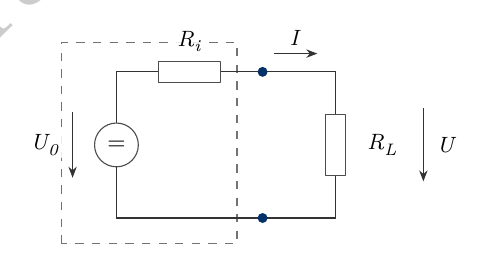
\begin{tikzpicture}[line join=round]
\filldraw[draw=black!55,dashed,fill=none] (1.221,-3.263) rectangle (3.448,-0.710);
\draw[black!80] (1.917,-2.938) -- (1.917,-1.082);
\draw[black!80] (1.917,-1.082) -- (4.701,-1.082);
\draw[black!80] (1.917,-2.938) -- (4.701,-2.938);
\draw[black!80] (4.701,-2.938) -- (4.701,-1.082);
\draw[draw=black!70,fill=white] (1.917,-2.010) circle (0.278);
\node[fill=white,fill opacity=0.85,text opacity=1,inner sep=1pt,font=\footnotesize] at (1.917,-2.010) {=};
\filldraw[draw=black!70,fill=white] (2.455,-1.212) rectangle (3.235,-0.952);
\filldraw[draw=black!70,fill=white] (4.571,-2.400) rectangle (4.831,-1.620);
\fill[FAUblue] (3.773,-1.082) circle (0.063);
\fill[FAUblue] (3.773,-2.938) circle (0.063);
\draw[-{Stealth[length=4pt]},black!80] (1.360,-1.592) -- (1.360,-2.427);
\node[anchor=east,fill=white,fill opacity=0.85,text opacity=1,inner sep=1pt,font=\footnotesize] at (1.234,-2.010) {\textit{U\textsubscript{0}}};
\node[fill=white,fill opacity=0.85,text opacity=1,inner sep=1pt,font=\footnotesize] at (2.845,-0.698) {\textit{R\textsubscript{i}}};
\draw[-{Stealth[length=4pt]},black!80] (3.912,-0.850) -- (4.469,-0.850);
\node[fill=white,fill opacity=0.85,text opacity=1,inner sep=1pt,font=\footnotesize] at (4.191,-0.652) {\textit{I}};
\node[anchor=west,fill=white,fill opacity=0.85,text opacity=1,inner sep=1pt,font=\footnotesize] at (5.059,-2.010) {\textit{R\textsubscript{L}}};
\draw[-{Stealth[length=4pt]},black!80] (5.815,-1.546) -- (5.815,-2.474);
\node[anchor=west,fill=white,fill opacity=0.85,text opacity=1,inner sep=1pt,font=\footnotesize] at (5.941,-2.010) {\textit{U}};
\end{tikzpicture}\par\smallskip{\small\raggedright \textbf{A real voltage source with a load.} Inside the dashed box an ideal source \textit{U}\textsubscript{0} sits in series with the internal resistance \textit{R}\textsubscript{i}. The load \textit{R}\textsubscript{L} only sees the two terminals (dots), where the voltage is \textit{U} = \textit{U}\textsubscript{0} \ensuremath{-} \textit{I}\textit{R}\textsubscript{i}.\par}\end{minipage}
\end{center}

\begin{equationcard}{Real current source}
\[ \begin{gathered} {I}\, =\, {I}_{0}\, -\, \dfrac{{U}}{{R}_{\mathrm{i}}} \\ {U}_{0}\, =\, {I}_{0}{R}_{\mathrm{i}} \end{gathered} \]
{\small \emph{Read it as: “the delivered current is I nought minus what the internal resistance takes”.}\par \textit{U}\textsubscript{0} is the open-circuit voltage. Here \textit{R}\textsubscript{i} sits in parallel with the ideal current source and takes the part \textit{I}\textsubscript{i} = {\small\ensuremath{\dfrac{{U}}{{R}_{\mathrm{i}}}}} of \textit{I}\textsubscript{0}. \textit{I}\textsubscript{0} is now the short-circuit current (\textit{U} = 0).}
\end{equationcard}
\end{keepsection}

\begin{keepsection}
\Needspace{12\baselineskip}
\subsection{Source transformation}

\begin{equationcard}{Equivalent real sources}
\[ \begin{gathered} {U}_{0}\, =\, {I}_{0}{R}_{\mathrm{i}} \\ \text{same}\, {R}_{\mathrm{i}}\, \text{in}\, \text{both}\, \text{models} \end{gathered} \]
{\small \emph{Read it as: “the voltage source equals the current source when U nought is I nought times R i”.}\par A real voltage source (\textit{U}\textsubscript{0} in series with \textit{R}\textsubscript{i}) and a real current source (\textit{I}\textsubscript{0} in parallel with the same \textit{R}\textsubscript{i}) give the same terminal line \textit{U} = \textit{U}\textsubscript{0} \ensuremath{-} \textit{I}\textit{R}\textsubscript{i}, so any load sees identical \textit{U} and \textit{I}. Inside they differ: with no load the voltage source wastes nothing, while the current source turns \textit{U}\textsubscript{0}\textit{I}\textsubscript{0} into heat in \textit{R}\textsubscript{i}; with a short circuit it is the other way round.}
\end{equationcard}
\end{keepsection}

\begin{keepsection}
\Needspace{11\baselineskip}
\subsection{Derivation: why the two models agree}

\Needspace{8\baselineskip}
\begin{enumerate}
\item Voltage model, KVL round source, \textit{R}\textsubscript{i} and terminals: \textit{U} = \textit{U}\textsubscript{0} \ensuremath{-} \textit{I}\textit{R}\textsubscript{i}.
\item Current model, KCL at the top node: \textit{I}\textsubscript{0} splits into \textit{I}\textsubscript{i} = {\small\ensuremath{\dfrac{{U}}{{R}_{\mathrm{i}}}}} through \textit{R}\textsubscript{i} and \textit{I} to the load, so \textit{I} = \textit{I}\textsubscript{0} \ensuremath{-} {\small\ensuremath{\dfrac{{U}}{{R}_{\mathrm{i}}}}}.
\item Multiply the second line by \textit{R}\textsubscript{i}: \textit{U} = \textit{I}\textsubscript{0}\textit{R}\textsubscript{i} \ensuremath{-} \textit{I}\textit{R}\textsubscript{i}.
\item This is the first line exactly when \textit{U}\textsubscript{0} = \textit{I}\textsubscript{0}\textit{R}\textsubscript{i}: both models then share one terminal line.
\end{enumerate}

\Needspace{14\baselineskip}
\begin{center}
\begin{minipage}[t]{0.950\linewidth}\centering
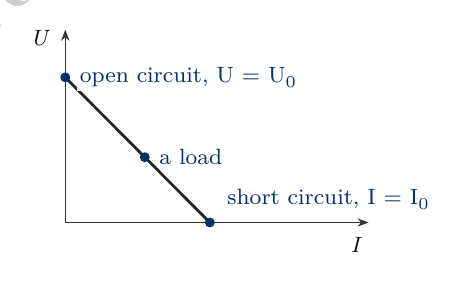
\begin{tikzpicture}[line join=round]
\draw[-{Stealth[length=4pt]},black!80] (0.720,-2.628) -- (4.572,-2.628);
\draw[-{Stealth[length=4pt]},black!80] (0.720,-2.628) -- (0.720,-0.180);
\draw[black!85,line width=1pt] (0.720,-0.785) -- (2.556,-2.628);
\fill[FAUblue] (0.720,-0.785) circle (0.063);
\node[anchor=west,text=FAUblue,fill=white,fill opacity=0.85,text opacity=1,inner sep=1pt,font=\footnotesize] at (0.864,-0.785) {open circuit, U = U\textsubscript{0}};
\fill[FAUblue] (2.556,-2.628) circle (0.063);
\node[anchor=west,text=FAUblue,inner sep=1pt,font=\footnotesize] at (2.737,-2.336) {short circuit, I = I\textsubscript{0}};
\fill[FAUblue] (1.730,-1.799) circle (0.063);
\node[anchor=west,text=FAUblue,fill=white,fill opacity=0.85,text opacity=1,inner sep=1pt,font=\footnotesize] at (1.874,-1.799) {a load};
\node[anchor=east,inner sep=1pt,font=\footnotesize] at (4.536,-2.916) {\textit{I}};
\node[anchor=east,inner sep=1pt,font=\footnotesize] at (0.576,-0.288) {\textit{U}};
\end{tikzpicture}\par\smallskip{\small\raggedright \textbf{The terminal line of a real source.} Every load picks one point on the same straight line from (\textit{U} = \textit{U}\textsubscript{0}, \textit{I} = 0) to (\textit{U} = 0, \textit{I} = \textit{I}\textsubscript{0}). Its slope is \ensuremath{-}\textit{R}\textsubscript{i}. Both models of §3.2 give exactly this line, which is why they can replace each other.\par}\end{minipage}
\end{center}

\begin{workedbox}{Worked example \ensuremath{\cdot} one battery, two models}
A battery has \textit{U}\textsubscript{0} = 12 V and \textit{R}\textsubscript{i} = 0.5 Ω and feeds a load \textit{R} = 5.5 Ω.

\Needspace{10\baselineskip}
\begin{enumerate}
\item Voltage-source model: \textit{I} = {\small\ensuremath{\dfrac{12\, \mathrm{V}}{0.5\, Ω\, +\, 5.5\, Ω}}} = 2 A and \textit{U} = 12 V \ensuremath{-} 2 A \ensuremath{\cdot} 0.5 Ω = 11 V.
\item Short-circuit current: \textit{I}\textsubscript{0} = {\small\ensuremath{\dfrac{12\, \mathrm{V}}{0.5\, Ω}}} = 24 A, so the current-source model is 24 A in parallel with 0.5 Ω.
\item Current-source model with the same load: the current divider (§3.5) sends \textit{I} = 24 A \ensuremath{\cdot} {\small\ensuremath{\dfrac{0.5\, Ω}{0.5\, Ω\, +\, 5.5\, Ω}}} = 2 A into the load, so \textit{U} = 2 A \ensuremath{\cdot} 5.5 Ω = 11 V.
\item Open terminals: the voltage-source model dissipates nothing, the current-source model 24 A \ensuremath{\cdot} 12 V = 288 W in its \textit{R}\textsubscript{i}.
\end{enumerate}

Check: both models give 2 A and 11 V at the load, and 11 V = 2 A \ensuremath{\cdot} 5.5 Ω. Only the internal losses differ, which is the point of the “keep in mind” remark in the notes.
\end{workedbox}
\end{keepsection}

\begin{keepsection}
\Needspace{13\baselineskip}
\subsection{Dependent sources}

\Needspace{10\baselineskip}
\begin{center}\small\begin{tabularx}{\linewidth}{>{\raggedright\arraybackslash}X>{\raggedright\arraybackslash}X>{\raggedright\arraybackslash}X>{\raggedright\arraybackslash}X}\toprule
\textbf{Type} & \textbf{Output} & \textbf{Controlled by} & \textbf{Factor and its unit} \\ \midrule
Voltage-controlled voltage source & \textit{U}\textsubscript{cd} = α\textit{U}\textsubscript{cg} & a voltage \textit{U}\textsubscript{cg} & α, no unit \\
Voltage-controlled current source & \textit{I}\textsubscript{cd} = β\textit{U}\textsubscript{cg} & a voltage \textit{U}\textsubscript{cg} & β in S \\
Current-controlled voltage source & \textit{U}\textsubscript{cd} = γ\textit{I}\textsubscript{cg} & a current \textit{I}\textsubscript{cg} & γ in Ω \\
Current-controlled current source & \textit{I}\textsubscript{cd} = δ\textit{I}\textsubscript{cg} & a current \textit{I}\textsubscript{cg} & δ, no unit \\
\bottomrule\end{tabularx}\end{center}

\Needspace{15\baselineskip}
Dependent sources are ideal and do not feed back on the controlling quantity, which can sit anywhere in the network. They use the same symbols as independent sources, with a function in place of a fixed value, and they model transistors and operational amplifiers in equivalent circuits. (The units of the factors follow directly from the output and control quantities; the notes do not list them.)

\begin{workedbox}{Worked example \ensuremath{\cdot} a voltage-controlled current source}
A model of an amplifier stage has a voltage-controlled current source with β = 20 mS, controlled by an input voltage \textit{U}\textsubscript{cg} = 0.5 V. Its output current flows through a 1 kΩ resistor.

\Needspace{5\baselineskip}
\begin{enumerate}
\item Output current: \textit{I}\textsubscript{cd} = β\textit{U}\textsubscript{cg} = 20 mS \ensuremath{\cdot} 0.5 V = 10 mA.
\item Output voltage across the resistor: 10 mA \ensuremath{\cdot} 1 kΩ = 10 V.
\item Voltage gain: {\small\ensuremath{\dfrac{10\, \mathrm{V}}{0.5\, \mathrm{V}}}} = 20.
\end{enumerate}

Check the units: S \ensuremath{\cdot} V = A and A \ensuremath{\cdot} Ω = V. Doubling the input doubles the output, because the source is linear.
\end{workedbox}

\Needspace{7\baselineskip}
\begin{notebox}\textbf{Trap:} \textit{I}\textsubscript{0} means different things: in a real current source it is the ideal source’s current, in a real voltage source it is the short-circuit current {\small\ensuremath{\dfrac{{U}_{0}}{{R}_{\mathrm{i}}}}}. After a transformation the two coincide, which is why the notes reuse the symbol.\end{notebox}

\Needspace{8\baselineskip}
\begin{notebox}\textbf{Sign check:} the terminal voltage of a real voltage source is never above \textit{U}\textsubscript{0} while it delivers current: \textit{U} = \textit{U}\textsubscript{0} \ensuremath{-} \textit{I}\textit{R}\textsubscript{i} with \textit{I} \ensuremath{\geq} 0.\end{notebox}

\Needspace{7\baselineskip}
\begin{notebox}\textbf{Near miss:} a 9 V source in parallel with a 3 Ω resistor looks like the transformation pattern, but it is not a real current source: an ideal voltage source in parallel with anything still fixes 9 V at the terminals, so the resistor changes nothing outside. The transformation needs \textit{R}\textsubscript{i} in series with a voltage source or in parallel with a current source.\end{notebox}

\Needspace{10\baselineskip}
\begin{recallbox}{Recall check \ensuremath{\cdot} answer before opening}
\Needspace{5\baselineskip}
\begin{enumerate}
\item A real voltage source has \textit{U}\textsubscript{0} = 6 V and \textit{I}\textsubscript{0} = 3 A. What is \textit{R}\textsubscript{i}?
\item Why may an ideal current source not be left open?
\item What is the unit of γ in a current-controlled voltage source?
\end{enumerate}

\nopagebreak[4]{\small\itshape Answers: see “3.2 Voltage and Current Sources” under Answers at the end.}
\end{recallbox}
\end{keepsection}
\end{keepsection}

\begin{keepsection}
\Needspace{13\baselineskip}
\section{3.3 Definitions, Network Graph}

\Needspace{10\baselineskip}
Before any law can be written down, every voltage and current needs a name and a direction. This section fixes the vocabulary and the sign conventions that §3.4 to §3.6 rely on.

\begin{plainbox}\textbf{In plain words:} \textbf{passive components} such as resistors use or store energy; \textbf{active components} such as sources feed it in. You reach a component only through its \textbf{terminals}. A pair of terminals is a \textbf{port} when the current going in at one equals the current coming out at the other. Strip a circuit down to its skeleton and you get a \textbf{network graph}: \textbf{branches} (the parts, as lines) meeting at \textbf{nodes} (dots), and closed paths through branches called \textbf{meshes}. Each branch voltage and current gets a \textbf{reference arrow}, the direction in which it counts as positive.\end{plainbox}

\begin{keepsection}
\Needspace{11\baselineskip}
\subsection{Terminals, ports and graphs}

\begin{equationcard}{Port condition}
\[ \begin{gathered} {I}_{1}'\, =\, {I}_{1} \end{gathered} \]
{\small \emph{Read it as: “the current leaving terminal 1 prime equals the current entering terminal 1”.}\par A two-terminal part is always a port, because what flows in must flow out (charge conservation from Chapter 2). A four-terminal part is a two-port when both terminal pairs meet the condition; once one pair does, the other does too.}
\end{equationcard}

\Needspace{10\baselineskip}
\begin{center}\small\begin{tabularx}{\linewidth}{>{\raggedright\arraybackslash}X>{\raggedright\arraybackslash}X>{\raggedright\arraybackslash}X}\toprule
\textbf{Term} & \textbf{Meaning} & \textbf{How to count it} \\ \midrule
Branch (b) & A two-terminal part of the network, one or more components & One line in the graph. A bare connecting wire is not a branch. \\
Node (n) & A terminal of a branch or a junction of several branches; it has one potential & Points joined only by wire are one node. \\
Mesh (m) & A closed sequence of branches through nodes & Write it as a list of branches, with a minus sign for a branch passed against its arrow. \\
\bottomrule\end{tabularx}\end{center}

\Needspace{14\baselineskip}
\begin{center}
\begin{minipage}[t]{0.950\linewidth}\centering
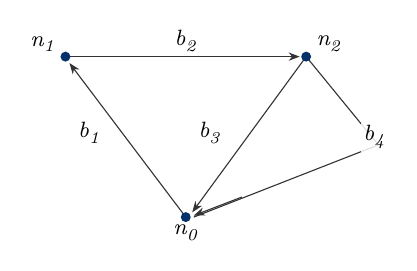
\begin{tikzpicture}[line join=round]
\draw[-{Stealth[length=4pt]},black!80] (2.877,-3.183) -- (1.400,-1.227);
\draw[-{Stealth[length=4pt]},black!80] (1.349,-1.145) -- (4.324,-1.145);
\draw[-{Stealth[length=4pt]},black!80] (4.406,-1.145) -- (2.959,-3.122);
\draw[black!80] (4.406,-1.145) -- (5.323,-2.266) -- (2.979,-3.183);
\draw[-{Stealth[length=4pt]},black!80] (3.590,-2.928) -- (2.979,-3.163);
\fill[FAUblue] (1.349,-1.145) circle (0.063);
\fill[FAUblue] (4.406,-1.145) circle (0.063);
\fill[FAUblue] (2.877,-3.183) circle (0.063);
\node[anchor=east,fill=white,fill opacity=0.85,text opacity=1,inner sep=1pt,font=\footnotesize] at (1.259,-0.983) {\textit{n\textsubscript{1}}};
\node[anchor=west,fill=white,fill opacity=0.85,text opacity=1,inner sep=1pt,font=\footnotesize] at (4.496,-0.983) {\textit{n\textsubscript{2}}};
\node[fill=white,fill opacity=0.85,text opacity=1,inner sep=1pt,font=\footnotesize] at (2.877,-3.381) {\textit{n\textsubscript{0}}};
\node[anchor=east,fill=white,fill opacity=0.85,text opacity=1,inner sep=1pt,font=\footnotesize] at (1.834,-2.113) {\textit{b\textsubscript{1}}};
\node[fill=white,fill opacity=0.85,text opacity=1,inner sep=1pt,font=\footnotesize] at (2.877,-0.947) {\textit{b\textsubscript{2}}};
\node[anchor=east,fill=white,fill opacity=0.85,text opacity=1,inner sep=1pt,font=\footnotesize] at (3.363,-2.113) {\textit{b\textsubscript{3}}};
\node[anchor=west,fill=white,fill opacity=0.85,text opacity=1,inner sep=1pt,font=\footnotesize] at (5.092,-2.164) {\textit{b\textsubscript{4}}};
\end{tikzpicture}\par\smallskip{\small\raggedright \textbf{A network graph.} The worked example’s circuit with every part drawn as a branch (line) between nodes (dots). The arrows give the reference direction of each branch current. Branches b\textsubscript{3} and b\textsubscript{4} join the same two nodes: that is a parallel connection.\par}\end{minipage}
\end{center}
\end{keepsection}

\begin{keepsection}
\Needspace{11\baselineskip}
\subsection{Reference arrows and sign conventions}

\begin{equationcard}{Reference directions}
\[ \begin{gathered} {U}_{12}\, =\, φ_{\mathrm{e}}(\mathrm{P}_{1})\, -\, φ_{\mathrm{e}}(\mathrm{P}_{2}) \end{gathered} \]
{\small \emph{Read it as: “U one two is the potential at P one minus the potential at P two”.}\par The voltage arrow points along the integration path of \textit{E}, from P\textsubscript{1} to P\textsubscript{2}; a current arrow points along the area element d\textit{A} used to compute it. Currents and voltages stay scalars: the arrow only tells you how to read the sign. A negative value means the actual direction is against the arrow.}
\end{equationcard}

\begin{equationcard}{Load and generator convention}
\[ \begin{gathered} {P}\, =\, {U}{I} \end{gathered} \]
{\small \emph{Read it as: “load: same direction, the part takes power; generator: opposite directions, the part gives power”.}\par Load convention: the \textit{U} and \textit{I} arrows point the same way through the part. Generator convention: they point opposite ways. Use the load convention for passive parts (then \textit{U} = \textit{R}\textit{I} with a plus sign) and the generator convention for sources. With the load convention \textit{P} \ensuremath{>} 0 means the part absorbs power; with the generator convention \textit{P} \ensuremath{>} 0 means it delivers power. (The power reading follows directly from \textit{P} = \textit{U}\textit{I} in Chapter 2; the notes describe it in words.) Fix one arrow freely; the convention then fixes the other.}
\end{equationcard}

\begin{workedbox}{Worked example \ensuremath{\cdot} counting and signs}
An ideal source \textit{U}\textsubscript{0} sits between nodes n\textsubscript{0} and n\textsubscript{1}; \textit{R}\textsubscript{1} joins n\textsubscript{1} to n\textsubscript{2}; \textit{R}\textsubscript{2} and \textit{R}\textsubscript{3} both join n\textsubscript{2} to n\textsubscript{0}.

\Needspace{9\baselineskip}
\begin{enumerate}
\item Nodes: n\textsubscript{0}, n\textsubscript{1}, n\textsubscript{2}, so three. Wire segments along the bottom all belong to n\textsubscript{0}.
\item Branches: the source, \textit{R}\textsubscript{1}, \textit{R}\textsubscript{2} and \textit{R}\textsubscript{3}, so four, as in the figure.
\item Meshes: for example (b\textsubscript{1}, b\textsubscript{2}, b\textsubscript{3}) round the left, and (b\textsubscript{3}, \ensuremath{-}b\textsubscript{4}) through the two parallel resistors.
\item A part measured with the load convention shows \textit{U} = 5 V and \textit{I} = \ensuremath{-}2 A. Then \textit{P} = \ensuremath{-}10 W: it delivers 10 W, so it acts as a source.
\end{enumerate}

Check: a mesh must end at the node where it started; (b\textsubscript{3}, \ensuremath{-}b\textsubscript{4}) goes n\textsubscript{2} \ensuremath{\to} n\textsubscript{0} along b\textsubscript{3} and back n\textsubscript{0} \ensuremath{\to} n\textsubscript{2} against b\textsubscript{4}’s arrow.
\end{workedbox}

\Needspace{5\baselineskip}
\begin{notebox}\textbf{Trap:} two dots joined only by a wire are one node, even if the drawing shows two. Count potentials, not dots.\end{notebox}

\Needspace{6\baselineskip}
\begin{notebox}\textbf{Memory hook:} load: arrows parallel, power in. Generator: arrows opposite, power out.\end{notebox}

\Needspace{11\baselineskip}
\begin{notebox}\textbf{Near miss:} a four-terminal box with 4 mA in at terminal 1 and 3 mA out at terminal 1\ensuremath{{}^{\prime}} is not a two-port: the missing 1 mA leaves through the other pair, so neither pair meets the port condition.\end{notebox}

\begin{recallbox}{Recall check \ensuremath{\cdot} answer before opening}
\Needspace{4\baselineskip}
\begin{enumerate}
\item How many nodes does a circuit have whose parts all connect between the same two wires?
\item A resistor’s current arrow points against its voltage arrow. What sign appears in Ohm’s law?
\end{enumerate}

\nopagebreak[4]{\small\itshape Answers: see “3.3 Definitions, Network Graph” under Answers at the end.}
\end{recallbox}
\end{keepsection}
\end{keepsection}

\begin{keepsection}
\Needspace{13\baselineskip}
\section{3.4 Kirchhoff’s Circuit Laws}

\Needspace{10\baselineskip}
Ohm’s law describes each part on its own; it says nothing about how parts are connected. Kirchhoff’s two laws supply exactly the missing equations, and they come straight from the field laws of Chapters 1 and 2.

\begin{plainbox}\textbf{In plain words:} walk round any closed loop of a circuit and add the potential steps: you end at the height you started from, so the steps add to zero. That is \textbf{Kirchhoff’s voltage law} (KVL). And at any junction, what flows in must flow out, because charge cannot pile up in a stationary current: \textbf{Kirchhoff’s current law} (KCL). Together with each part’s current–voltage rule, these give enough equations to find every unknown.\end{plainbox}

\begin{keepsection}
\Needspace{10\baselineskip}
\subsection{Kirchhoff’s voltage law}

\begin{equationcard}{KVL}
\[ \begin{gathered} \sum_{μ\, \in \, \text{mesh}}^{} \, {U}_{μ}\, =\, 0 \end{gathered} \]
{\small \emph{Read it as: “the sum of the branch voltages round a mesh is zero”.}\par Go round the mesh in either direction. A voltage whose arrow points along the direction of travel counts +, one against it counts \ensuremath{-}. The mesh need not follow wires: a voltage between two unconnected points (such as an unknown \textit{U}\textsubscript{x}) can close it.}
\end{equationcard}
\end{keepsection}

\begin{keepsection}
\Needspace{11\baselineskip}
\subsection{Derivation: KVL from the field}

\Needspace{8\baselineskip}
\begin{enumerate}
\item The electrostatic field has no circulation: $\oint $ \textit{E} \ensuremath{\cdot} d\textit{s} = 0 round any closed path (Chapter 1).
\item Split the path at the nodes P\textsubscript{1}, P\textsubscript{2}, …, P\textsubscript{\textit{k}} it passes. Each piece is a potential difference, for example φ\textsubscript{P1} \ensuremath{-} φ\textsubscript{P2}, which is the branch voltage between those nodes, with a minus sign when its arrow points against the travel.
\item The sum of the pieces telescopes, (φ\textsubscript{P1} \ensuremath{-} φ\textsubscript{P2}) + (φ\textsubscript{P2} \ensuremath{-} φ\textsubscript{P3}) + … + (φ\textsubscript{P\textit{k}} \ensuremath{-} φ\textsubscript{P1}) = 0, which is \ensuremath{\textstyle\sum} \textit{U}\textsubscript{μ} = 0.
\end{enumerate}

\Needspace{14\baselineskip}
\begin{center}
\begin{minipage}[t]{0.950\linewidth}\centering
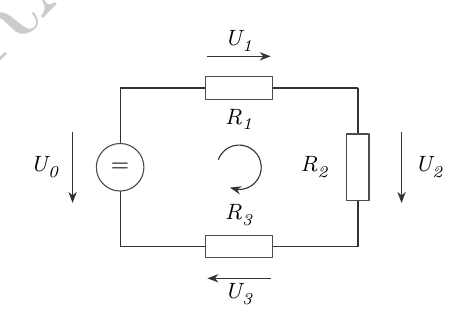
\begin{tikzpicture}[line join=round]
\draw[black!80] (1.942,-3.251) -- (1.942,-1.237);
\draw[black!80] (1.942,-1.237) -- (4.963,-1.237);
\draw[black!80] (4.963,-1.237) -- (4.963,-3.251);
\draw[black!80] (4.963,-3.251) -- (1.942,-3.251);
\draw[draw=black!70,fill=white] (1.942,-2.244) circle (0.302);
\node[fill=white,fill opacity=0.85,text opacity=1,inner sep=1pt,font=\footnotesize] at (1.942,-2.244) {=};
\filldraw[draw=black!70,fill=white] (3.029,-1.378) rectangle (3.875,-1.096);
\filldraw[draw=black!70,fill=white] (4.822,-2.667) rectangle (5.103,-1.821);
\filldraw[draw=black!70,fill=white] (3.029,-3.392) rectangle (3.875,-3.110);
\draw[-{Stealth[length=4pt]},black!80] (1.338,-1.791) -- (1.338,-2.697);
\node[anchor=east,fill=white,fill opacity=0.85,text opacity=1,inner sep=1pt,font=\footnotesize] at (1.212,-2.244) {\textit{U\textsubscript{0}}};
\draw[-{Stealth[length=4pt]},black!80] (3.050,-0.835) -- (3.855,-0.835);
\node[fill=white,fill opacity=0.85,text opacity=1,inner sep=1pt,font=\footnotesize] at (3.452,-0.637) {\textit{U\textsubscript{1}}};
\node[fill=white,fill opacity=0.85,text opacity=1,inner sep=1pt,font=\footnotesize] at (3.452,-1.637) {\textit{R\textsubscript{1}}};
\draw[-{Stealth[length=4pt]},black!80] (5.516,-1.791) -- (5.516,-2.697);
\node[anchor=west,fill=white,fill opacity=0.85,text opacity=1,inner sep=1pt,font=\footnotesize] at (5.642,-2.244) {\textit{U\textsubscript{2}}};
\node[anchor=east,fill=white,fill opacity=0.85,text opacity=1,inner sep=1pt,font=\footnotesize] at (4.635,-2.244) {\textit{R\textsubscript{2}}};
\draw[-{Stealth[length=4pt]},black!80] (3.855,-3.654) -- (3.050,-3.654);
\node[fill=white,fill opacity=0.85,text opacity=1,inner sep=1pt,font=\footnotesize] at (3.452,-3.852) {\textit{U\textsubscript{3}}};
\node[fill=white,fill opacity=0.85,text opacity=1,inner sep=1pt,font=\footnotesize] at (3.452,-2.852) {\textit{R\textsubscript{3}}};
\draw[black!80] (3.188,-2.148) -- (3.212,-2.098) -- (3.245,-2.054) -- (3.285,-2.017) -- (3.334,-1.988) -- (3.385,-1.970) -- (3.440,-1.962) -- (3.496,-1.965) -- (3.549,-1.979) -- (3.598,-2.004) -- (3.643,-2.037) -- (3.680,-2.077) -- (3.708,-2.125) -- (3.726,-2.177) -- (3.734,-2.232) -- (3.731,-2.287) -- (3.717,-2.341) -- (3.693,-2.390) -- (3.660,-2.434) -- (3.619,-2.472) -- (3.571,-2.500) -- (3.520,-2.518) -- (3.464,-2.526) -- (3.409,-2.523) -- (3.356,-2.509);
\draw[-{Stealth[length=4pt]},black!80] (3.423,-2.524) -- (3.338,-2.502);
\end{tikzpicture}\par\smallskip{\small\raggedright \textbf{One mesh, traversed clockwise.} \textit{U}\textsubscript{1}, \textit{U}\textsubscript{2} and \textit{U}\textsubscript{3} point along the direction of travel and count with a plus sign; \textit{U}\textsubscript{0} points against it and counts with a minus sign: \ensuremath{-}\textit{U}\textsubscript{0} + \textit{U}\textsubscript{1} + \textit{U}\textsubscript{2} + \textit{U}\textsubscript{3} = 0.\par}\end{minipage}
\end{center}

\begin{workedbox}{Worked example \ensuremath{\cdot} an unknown voltage in a mesh}
In the figure \textit{U}\textsubscript{0} = 12 V, \textit{U}\textsubscript{1} = 3 V and \textit{U}\textsubscript{2} = 5 V. Find \textit{U}\textsubscript{3}.

\Needspace{5\baselineskip}
\begin{enumerate}
\item Travel clockwise. Against the travel: \textit{U}\textsubscript{0}. Along it: \textit{U}\textsubscript{1}, \textit{U}\textsubscript{2}, \textit{U}\textsubscript{3}.
\item KVL: \ensuremath{-}\textit{U}\textsubscript{0} + \textit{U}\textsubscript{1} + \textit{U}\textsubscript{2} + \textit{U}\textsubscript{3} = 0.
\item \textit{U}\textsubscript{3} = 12 V \ensuremath{-} 3 V \ensuremath{-} 5 V = 4 V.
\end{enumerate}

Check: the source’s 12 V is shared out among the three resistors, 3 + 5 + 4 = 12. A negative result would have meant \textit{U}\textsubscript{3} points the other way.
\end{workedbox}
\end{keepsection}

\begin{keepsection}
\Needspace{11\baselineskip}
\subsection{Kirchhoff’s current law}

\begin{equationcard}{KCL}
\[ \begin{gathered} \sum_{μ\, \in \, \text{node}}^{} \, {I}_{μ}\, =\, 0 \end{gathered} \]
{\small \emph{Read it as: “the sum of the currents at a node is zero”.}\par Count a current + when its arrow points into the node and \ensuremath{-} when it points out (or the other way round, consistently). The node may be a closed surface round a whole region of the circuit: the currents crossing the surface still add to zero. Of the equations for all \textit{N} nodes, one is always redundant.}
\end{equationcard}
\end{keepsection}

\begin{keepsection}
\Needspace{10\baselineskip}
\subsection{Derivation: KCL from charge conservation}

\Needspace{7\baselineskip}
\begin{enumerate}
\item For stationary currents the charge inside any closed surface stays constant, so $\oiint $ \textit{J} \ensuremath{\cdot} d\textit{A} = 0 (Chapter 2).
\item Put the surface round a node. It cuts only the wires that meet there, and the flux through each wire’s cross-section is that wire’s current, + for an inward arrow and \ensuremath{-} for an outward one.
\item The flux integral becomes \ensuremath{\textstyle\sum} \textit{I}\textsubscript{μ} = 0: inflow equals outflow.
\end{enumerate}

\begin{workedbox}{Worked example \ensuremath{\cdot} currents at a node and round a region}
At a node, 3 A flows in on wire 1, 1.2 A flows out on wire 2, and wire 3 carries \ensuremath{-}0.8 A with its arrow pointing in. Wire 4’s arrow points out.

\Needspace{6\baselineskip}
\begin{enumerate}
\item KCL with inward arrows +: 3 A \ensuremath{-} 1.2 A + (\ensuremath{-}0.8 A) \ensuremath{-} \textit{I}\textsubscript{4} = 0.
\item \textit{I}\textsubscript{4} = 1.0 A, flowing out as its arrow says.
\item Wire 3’s negative value means 0.8 A actually leaves the node; KCL handles that without redrawing the arrow.
\end{enumerate}

Check by actual directions: in 3 A; out 1.2 + 0.8 + 1.0 = 3 A.
\end{workedbox}

\Needspace{6\baselineskip}
\begin{notebox}\textbf{Trap:} sign errors come from the arrows, not the values. Decide the travel direction (KVL) or the in/out rule (KCL) first, write the signs, and only then insert numbers.\end{notebox}

\Needspace{7\baselineskip}
\begin{notebox}\textbf{Sign check:} an ideal current source in a mesh still has a voltage; it is just unknown. KVL is how you find it.\end{notebox}

\Needspace{6\baselineskip}
\begin{notebox}\textbf{Near miss:} a 2 A current source drives a loop through a 5 Ω resistor and a 4 V ideal voltage source whose + terminal the current enters. Setting the current source’s voltage to zero breaks KVL (10 V + 4 V \ensuremath{\neq} 0). Its voltage is the unknown that closes the loop: 14 V.\end{notebox}

\Needspace{10\baselineskip}
\begin{recallbox}{Recall check \ensuremath{\cdot} answer before opening}
\Needspace{5\baselineskip}
\begin{enumerate}
\item What field law is KVL a consequence of?
\item A closed surface encloses half a circuit. What do the crossing currents add up to?
\item How many independent KCL equations does a network with 4 nodes give?
\end{enumerate}

\nopagebreak[4]{\small\itshape Answers: see “3.4 Kirchhoff’s Circuit Laws” under Answers at the end.}
\end{recallbox}
\end{keepsection}
\end{keepsection}

\begin{keepsection}
\Needspace{14\baselineskip}
\section{3.5 Simple Resistor Networks}

\Needspace{11\baselineskip}
With Kirchhoff’s laws (§3.4) every network can be solved, but most of the time a few parts can be merged first. Series and parallel rules, dividers and the source–load relations are the shortcuts you will use in almost every problem.

\begin{plainbox}\textbf{In plain words:} parts in \textbf{series} carry the same current, one after another like beads on a string; parts in \textbf{parallel} share the same voltage, side by side like lanes of a road. A \textbf{voltage divider} uses a series chain to tap off part of a voltage; a \textbf{current divider} uses parallel branches to split a current. Attaching something to a divider \textbf{loads} it and changes the split. Finally, a real source delivers the most power when the load matches its internal resistance (\textbf{maximum power transfer}), but then half the power is lost inside, so the \textbf{efficiency} is only 50 \%.\end{plainbox}

\begin{keepsection}
\Needspace{9\baselineskip}
\subsection{Series and parallel}

\begin{equationcard}{Series connection}
\[ \begin{gathered} {R}_{\text{total}}\, =\, \sum_{{n}=1}^{{N}} \, {R}_{{n}} \end{gathered} \]
{\small \emph{Read it as: “in series the resistances add”.}\par Same current through every resistor; the voltages add (KVL). \textit{R}\textsubscript{total} is larger than the largest single resistance.}
\end{equationcard}

\begin{equationcard}{Parallel connection}
\[ \begin{gathered} {G}_{\text{total}}\, =\, \sum_{{n}=1}^{{N}} \, {G}_{{n}} \\ {R}_{1}\, \parallel \, {R}_{2}\, =\, \dfrac{1}{\dfrac{1}{{R}_{1}}\, +\, \dfrac{1}{{R}_{2}}}\, =\, \dfrac{{R}_{1}{R}_{2}}{{R}_{1}\, +\, {R}_{2}} \end{gathered} \]
{\small \emph{Read it as: “in parallel the conductances add; two resistors give product over sum”.}\par Same voltage across every resistor; the currents add (KCL). \textit{R}\textsubscript{total} is smaller than the smallest single resistance; \textit{N} equal resistors \textit{R} in parallel give {\small\ensuremath{\dfrac{{R}}{{N}}}}. The symbol \ensuremath{\parallel} is the parallel operator; the product-over-sum form only works for two resistors at a time. These rules are dual to those for capacitors, which add in parallel.}
\end{equationcard}
\end{keepsection}

\begin{keepsection}
\Needspace{10\baselineskip}
\subsection{Derivation: series and parallel}

\Needspace{7\baselineskip}
\begin{enumerate}
\item Series: one current \textit{I} flows through every resistor, and KVL adds the voltages: \textit{U}\textsubscript{total} = \ensuremath{\textstyle\sum} \textit{R}\textsubscript{\textit{n}}\textit{I}. Dividing by \textit{I} gives \textit{R}\textsubscript{total} = \ensuremath{\textstyle\sum} \textit{R}\textsubscript{\textit{n}}.
\item Parallel: one voltage \textit{U} lies across every resistor, and KCL adds the currents: \textit{I}\textsubscript{total} = \ensuremath{\textstyle\sum} {\small\ensuremath{\dfrac{{U}}{{R}_{{n}}}}} = \textit{U} \ensuremath{\textstyle\sum} \textit{G}\textsubscript{\textit{n}}. Dividing by \textit{U} gives \textit{G}\textsubscript{total} = \ensuremath{\textstyle\sum} \textit{G}\textsubscript{\textit{n}}.
\item Two resistors: {\small\ensuremath{\dfrac{1}{\dfrac{1}{{R}_{1}}\, +\, \dfrac{1}{{R}_{2}}}}} = {\small\ensuremath{\dfrac{{R}_{1}{R}_{2}}{{R}_{2}\, +\, {R}_{1}}}}, multiplying top and bottom by \textit{R}\textsubscript{1}\textit{R}\textsubscript{2}.
\end{enumerate}

\begin{workedbox}{Worked example \ensuremath{\cdot} reduce a network step by step}
A 6 Ω resistor is in series with a parallel pair of 12 Ω and 4 Ω, and the chain is connected to 18 V.

\Needspace{7\baselineskip}
\begin{enumerate}
\item Parallel pair: 12 Ω \ensuremath{\parallel} 4 Ω = {\small\ensuremath{\dfrac{12\, \cdot \, 4}{12\, +\, 4}}} Ω = 3 Ω.
\item Series with 6 Ω: \textit{R}\textsubscript{total} = 9 Ω, so the current from the source is {\small\ensuremath{\dfrac{18\, \mathrm{V}}{9\, Ω}}} = 2 A.
\item Voltage across the pair: 2 A \ensuremath{\cdot} 3 Ω = 6 V; across the 6 Ω resistor: 12 V.
\item Branch currents: {\small\ensuremath{\dfrac{6\, \mathrm{V}}{12\, Ω}}} = 0.5 A and {\small\ensuremath{\dfrac{6\, \mathrm{V}}{4\, Ω}}} = 1.5 A.
\end{enumerate}

Check: 0.5 A + 1.5 A = 2 A (KCL) and 12 V + 6 V = 18 V (KVL). The 3 Ω result is below the smaller resistor, 4 Ω, as a parallel result must be.
\end{workedbox}
\end{keepsection}

\begin{keepsection}
\Needspace{11\baselineskip}
\subsection{Voltage divider}

\begin{equationcard}{Unloaded voltage divider}
\[ \begin{gathered} \dfrac{{U}_{{n}}}{{U}_{\text{total}}}\, =\, \dfrac{{R}_{{n}}}{{R}_{\text{total}}} \\ \dfrac{{U}_{{k}}}{{U}_{{n}}}\, =\, \dfrac{{R}_{{k}}}{{R}_{{n}}} \\ \text{two}\, \text{resistors}:\, {U}_{2}\, =\, \dfrac{{R}_{2}}{{R}_{1}\, +\, {R}_{2}}\, {U} \end{gathered} \]
{\small \emph{Read it as: “each part of the voltage is in the same ratio to the total as its resistance is to the total”.}\par Only for a series chain, where one current flows through every resistor: each resistor takes a share of the voltage in proportion to its resistance.}
\end{equationcard}

\begin{equationcard}{Loaded voltage divider}
\[ \begin{gathered} {R}_{\text{par}}\, =\, {R}_{2}\, \parallel \, {R}_{\mathrm{L}}\, =\, \dfrac{{R}_{2}{R}_{\mathrm{L}}}{{R}_{2}\, +\, {R}_{\mathrm{L}}} \\ \dfrac{{U}_{2}}{{U}}\, =\, \dfrac{{R}_{\text{par}}}{{R}_{1}\, +\, {R}_{\text{par}}}\, =\, \dfrac{{R}_{2}{R}_{\mathrm{L}}}{{R}_{1}{R}_{2}\, +\, {R}_{\mathrm{L}}({R}_{1}\, +\, {R}_{2})} \end{gathered} \]
{\small \emph{Read it as: “U two over U is R par over R one plus R par”.}\par A load \textit{R}\textsubscript{L} at the tap draws \textit{I}\textsubscript{L}, so \textit{R}\textsubscript{2} no longer carries the full current and the unloaded ratio fails. Combine \textit{R}\textsubscript{2} with \textit{R}\textsubscript{L} first; the result is again an unloaded divider. For \textit{R}\textsubscript{L} \ensuremath{\to} \ensuremath{\infty} it returns to {\small\ensuremath{\dfrac{{R}_{2}}{{R}_{1}\, +\, {R}_{2}}}}. Keep \textit{R}\textsubscript{L} large compared with \textit{R}\textsubscript{2} if the tap voltage must not sag.}
\end{equationcard}
\end{keepsection}

\begin{keepsection}
\Needspace{11\baselineskip}
\subsection{Derivation: unloaded and loaded divider}

\Needspace{8\baselineskip}
\begin{enumerate}
\item Unloaded: one current \textit{I} = {\small\ensuremath{\dfrac{{U}}{{R}_{1}\, +\, {R}_{2}}}} flows through both, so \textit{U}\textsubscript{2} = \textit{R}\textsubscript{2}\textit{I} = {\small\ensuremath{\dfrac{{R}_{2}}{{R}_{1}\, +\, {R}_{2}}}} \textit{U}.
\item Loaded: \textit{R}\textsubscript{L} is in parallel with \textit{R}\textsubscript{2}, so replace \textit{R}\textsubscript{2} by \textit{R}\textsubscript{par} = {\small\ensuremath{\dfrac{{R}_{2}{R}_{\mathrm{L}}}{{R}_{2}\, +\, {R}_{\mathrm{L}}}}} and use the unloaded rule: {\small\ensuremath{\dfrac{{U}_{2}}{{U}}}} = {\small\ensuremath{\dfrac{{R}_{\text{par}}}{{R}_{1}\, +\, {R}_{\text{par}}}}}.
\item Multiply top and bottom by (\textit{R}\textsubscript{2} + \textit{R}\textsubscript{L}): {\small\ensuremath{\dfrac{{U}_{2}}{{U}}}} = {\small\ensuremath{\dfrac{{R}_{2}{R}_{\mathrm{L}}}{{R}_{1}({R}_{2}\, +\, {R}_{\mathrm{L}})\, +\, {R}_{2}{R}_{\mathrm{L}}}}} = {\small\ensuremath{\dfrac{{R}_{2}{R}_{\mathrm{L}}}{{R}_{1}{R}_{2}\, +\, {R}_{\mathrm{L}}({R}_{1}\, +\, {R}_{2})}}}.
\item For \textit{R}\textsubscript{L} \ensuremath{\to} \ensuremath{\infty} divide top and bottom by \textit{R}\textsubscript{L}: the ratio tends to {\small\ensuremath{\dfrac{{R}_{2}}{{R}_{1}\, +\, {R}_{2}}}}, the unloaded value.
\end{enumerate}

\Needspace{14\baselineskip}
\begin{center}
\begin{minipage}[t]{0.950\linewidth}\centering
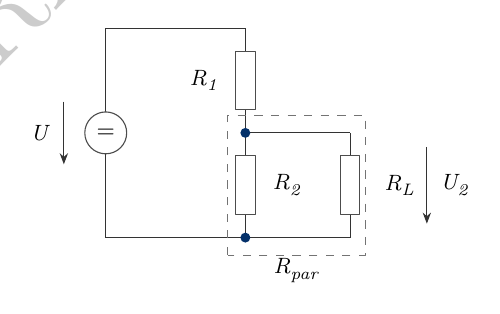
\begin{tikzpicture}[line join=round]
\draw[black!80] (1.762,-3.446) -- (1.762,-0.787);
\draw[black!80] (1.762,-0.787) -- (3.535,-0.787);
\draw[black!80] (3.535,-0.787) -- (3.535,-3.446);
\draw[black!80] (1.762,-3.446) -- (4.865,-3.446);
\draw[black!80] (3.535,-2.116) -- (4.865,-2.116);
\draw[black!80] (4.865,-2.116) -- (4.865,-3.446);
\draw[draw=black!70,fill=white] (1.762,-2.116) circle (0.266);
\node[fill=white,fill opacity=0.85,text opacity=1,inner sep=1pt,font=\footnotesize] at (1.762,-2.116) {=};
\filldraw[draw=black!70,fill=white] (3.411,-1.824) rectangle (3.659,-1.079);
\filldraw[draw=black!70,fill=white] (3.411,-3.154) rectangle (3.659,-2.409);
\filldraw[draw=black!70,fill=white] (4.741,-3.154) rectangle (4.989,-2.409);
\fill[FAUblue] (3.535,-2.116) circle (0.063);
\fill[FAUblue] (3.535,-3.446) circle (0.063);
\draw[-{Stealth[length=4pt]},black!80] (1.230,-1.718) -- (1.230,-2.515);
\node[anchor=east,fill=white,fill opacity=0.85,text opacity=1,inner sep=1pt,font=\footnotesize] at (1.104,-2.116) {\textit{U}};
\node[anchor=east,fill=white,fill opacity=0.85,text opacity=1,inner sep=1pt,font=\footnotesize] at (3.232,-1.452) {\textit{R\textsubscript{1}}};
\node[anchor=west,fill=white,fill opacity=0.85,text opacity=1,inner sep=1pt,font=\footnotesize] at (3.838,-2.781) {\textit{R\textsubscript{2}}};
\node[anchor=west,fill=white,fill opacity=0.85,text opacity=1,inner sep=1pt,font=\footnotesize] at (5.257,-2.781) {\textit{R\textsubscript{L}}};
\draw[-{Stealth[length=4pt]},black!80] (5.840,-2.294) -- (5.840,-3.269);
\node[anchor=west,fill=white,fill opacity=0.85,text opacity=1,inner sep=1pt,font=\footnotesize] at (5.966,-2.781) {\textit{U\textsubscript{2}}};
\filldraw[draw=black!55,dashed,fill=none] (3.313,-3.668) rectangle (5.060,-1.895);
\node[fill=white,fill opacity=0.85,text opacity=1,inner sep=1pt,font=\footnotesize] at (4.182,-3.866) {\textit{R\textsubscript{par}}};
\end{tikzpicture}\par\smallskip{\small\raggedright \textbf{A loaded voltage divider.} The load \textit{R}\textsubscript{L} at the tap sits in parallel with \textit{R}\textsubscript{2}; together (dashed box) they form \textit{R}\textsubscript{par} = \textit{R}\textsubscript{2} \ensuremath{\parallel} \textit{R}\textsubscript{L}, which is smaller than \textit{R}\textsubscript{2}. The divider is now \textit{R}\textsubscript{1} over \textit{R}\textsubscript{par}, so \textit{U}\textsubscript{2} drops below its unloaded value.\par}\end{minipage}
\end{center}

\begin{workedbox}{Worked example \ensuremath{\cdot} how much a load pulls down a divider}
\textit{U} = 12 V and \textit{R}\textsubscript{1} = \textit{R}\textsubscript{2} = 10 kΩ.

\Needspace{5\baselineskip}
\begin{enumerate}
\item Unloaded: \textit{U}\textsubscript{2} = 12 V \ensuremath{\cdot} {\small\ensuremath{\dfrac{10\, \mathrm{k}Ω}{20\, \mathrm{k}Ω}}} = 6 V.
\item Load \textit{R}\textsubscript{L} = 10 kΩ: \textit{R}\textsubscript{par} = 10 kΩ \ensuremath{\parallel} 10 kΩ = 5 kΩ, so \textit{U}\textsubscript{2} = 12 V \ensuremath{\cdot} {\small\ensuremath{\dfrac{5\, \mathrm{k}Ω}{15\, \mathrm{k}Ω}}} = 4 V.
\item Load \textit{R}\textsubscript{L} = 1 MΩ: \textit{R}\textsubscript{par} = {\small\ensuremath{\dfrac{10\, \cdot \, 1000}{1010}}} kΩ \ensuremath{\approx} 9.90 kΩ, so \textit{U}\textsubscript{2} \ensuremath{\approx} 12 V \ensuremath{\cdot} {\small\ensuremath{\dfrac{9.90}{19.90}}} \ensuremath{\approx} 5.97 V.
\end{enumerate}

Check with the closed formula for \textit{R}\textsubscript{L} = 10 kΩ: {\small\ensuremath{\dfrac{10\, \cdot \, 10}{10\, \cdot \, 10\, +\, 10\, \cdot \, 20}}} = {\small\ensuremath{\dfrac{1}{3}}}, and 12 V \ensuremath{\cdot} {\small\ensuremath{\dfrac{1}{3}}} = 4 V. A load a hundred times \textit{R}\textsubscript{2} costs only 0.5 \%.
\end{workedbox}
\end{keepsection}

\begin{keepsection}
\Needspace{11\baselineskip}
\subsection{Current divider}

\begin{equationcard}{Unloaded current divider}
\[ \begin{gathered} \dfrac{{I}_{{n}}}{{I}_{\text{total}}}\, =\, \dfrac{{G}_{{n}}}{{G}_{\text{total}}} \\ \text{two}\, \text{resistors}:\, \dfrac{{I}_{1}}{{I}_{2}}\, =\, \dfrac{{R}_{2}}{{R}_{1}},\, \dfrac{{I}_{2}}{{I}}\, =\, \dfrac{{R}_{1}}{{R}_{1}\, +\, {R}_{2}} \end{gathered} \]
{\small \emph{Read it as: “each branch current is in the same ratio to the total as its conductance is to the total”.}\par Only for parallel branches with one shared voltage: each branch takes a share of the current in proportion to its conductance. With two resistors the larger current flows through the smaller resistance, so the formula has the other resistor on top.}
\end{equationcard}

\begin{equationcard}{Loaded current divider}
\[ \begin{gathered} \dfrac{{I}_{2}}{{I}}\, =\, \dfrac{{R}_{1}}{{R}_{1}\, +\, {R}_{2}\, +\, {R}_{\mathrm{L}}} \end{gathered} \]
{\small \emph{Read it as: “I two over I is R one over the sum of all three”.}\par A load \textit{R}\textsubscript{L} in series with \textit{R}\textsubscript{2} forms \textit{R}\textsubscript{ser} = \textit{R}\textsubscript{2} + \textit{R}\textsubscript{L}; then the two-resistor rule applies with \textit{R}\textsubscript{ser} in place of \textit{R}\textsubscript{2}.}
\end{equationcard}
\end{keepsection}

\begin{keepsection}
\Needspace{8\baselineskip}
\subsection{Derivation: current divider}

\Needspace{5\baselineskip}
\begin{enumerate}
\item One voltage across both branches: \textit{U} = {\small\ensuremath{\dfrac{{I}}{{G}_{1}\, +\, {G}_{2}}}}, from KCL \textit{I} = \textit{G}\textsubscript{1}\textit{U} + \textit{G}\textsubscript{2}\textit{U}.
\item Branch current: \textit{I}\textsubscript{2} = \textit{G}\textsubscript{2}\textit{U} = {\small\ensuremath{\dfrac{{G}_{2}}{{G}_{1}\, +\, {G}_{2}}}} \textit{I} = {\small\ensuremath{\dfrac{{R}_{1}}{{R}_{1}\, +\, {R}_{2}}}} \textit{I}, multiplying top and bottom by \textit{R}\textsubscript{1}\textit{R}\textsubscript{2}.
\item Loaded: \textit{R}\textsubscript{2} and \textit{R}\textsubscript{L} are in series, so use \textit{R}\textsubscript{ser} = \textit{R}\textsubscript{2} + \textit{R}\textsubscript{L} in place of \textit{R}\textsubscript{2}: {\small\ensuremath{\dfrac{{I}_{2}}{{I}}}} = {\small\ensuremath{\dfrac{{R}_{1}}{{R}_{1}\, +\, {R}_{2}\, +\, {R}_{\mathrm{L}}}}}.
\end{enumerate}

\begin{workedbox}{Worked example \ensuremath{\cdot} measuring range of an ammeter}
A meter has internal resistance 5 Ω and reads at most 10 mA. It must measure up to 0.5 A.

\Needspace{5\baselineskip}
\begin{enumerate}
\item The meter may carry {\small\ensuremath{\dfrac{10\, \text{mA}}{0.5\, \mathrm{A}}}} = {\small\ensuremath{\dfrac{1}{50}}} of the current, so \textit{G}\textsubscript{total} = 50 \ensuremath{\cdot} \textit{G}\textsubscript{i} = 50 \ensuremath{\cdot} 0.2 S = 10 S.
\item Shunt: \textit{G}\textsubscript{par} = 10 S \ensuremath{-} 0.2 S = 9.8 S, so \textit{R}\textsubscript{par} = {\small\ensuremath{\dfrac{1}{9.8\, \mathrm{S}}}} \ensuremath{\approx} 0.102 Ω.
\item Reading: the true current is 50 times the meter current.
\end{enumerate}

Check: at full scale 10 mA \ensuremath{\cdot} 5 Ω = 50 mV across the meter, and the shunt carries {\small\ensuremath{\dfrac{50\, \text{mV}}{0.102\, Ω}}} \ensuremath{\approx} 490 mA; together 0.5 A. A voltmeter is extended the other way, with a series resistor that takes the extra voltage.
\end{workedbox}
\end{keepsection}

\begin{keepsection}
\Needspace{11\baselineskip}
\subsection{Sources and loads: power and efficiency}

\begin{equationcard}{Power from a real voltage source}
\[ \begin{gathered} {P}_{\text{total}}\, =\, {U}_{0}{I}\, =\, \dfrac{{U}_{0}^{2}}{{R}_{\mathrm{i}}\, +\, {R}_{\mathrm{L}}} \\ {P}_{\mathrm{L}}\, =\, \dfrac{{U}^{2}}{{R}_{\mathrm{L}}}\, =\, {U}_{0}^{2}\, \dfrac{{R}_{\mathrm{L}}}{({R}_{\mathrm{i}}\, +\, {R}_{\mathrm{L}})^{2}} \end{gathered} \]
{\small \emph{Read it as: “the load power is U nought squared times R L over the square of the total resistance”.}\par \textit{P}\textsubscript{total} is what the ideal source supplies, \textit{P}\textsubscript{L} what reaches the load. \textit{P}\textsubscript{L} \ensuremath{\to} 0 both for an open circuit (\textit{R}\textsubscript{L} \ensuremath{\to} \ensuremath{\infty}, no current) and a short circuit (\textit{R}\textsubscript{L} \ensuremath{\to} 0, no voltage), so it has a maximum in between.}
\end{equationcard}

\begin{equationcard}{Maximum power transfer and efficiency}
\[ \begin{gathered} {R}_{\mathrm{L}}\, =\, {R}_{\mathrm{i}}\, \Rightarrow \, {P}_{\mathrm{L},\text{max}}\, =\, \dfrac{{U}_{0}^{2}}{4{R}_{\mathrm{i}}} \\ {η}\, =\, \dfrac{{P}_{\mathrm{L}}}{{P}_{\text{total}}}\, =\, \dfrac{{R}_{\mathrm{L}}}{{R}_{\mathrm{i}}\, +\, {R}_{\mathrm{L}}} \end{gathered} \]
{\small \emph{Read it as: “the most power reaches the load when R L equals R i, and then the efficiency is one half”.}\par Setting {\small\ensuremath{\dfrac{\mathrm{d}{P}_{\mathrm{L}}}{\mathrm{d}{R}_{\mathrm{L}}}}} = 0 gives \textit{R}\textsubscript{L} = \textit{R}\textsubscript{i}. At that point the internal resistance heats up exactly as much as the load receives, so \textit{η} = 50 \%. High efficiency needs \textit{R}\textsubscript{L} \ensuremath{\gg} \textit{R}\textsubscript{i}: power engineering wants efficiency, signal and communications engineering wants maximum power.}
\end{equationcard}
\end{keepsection}

\begin{keepsection}
\Needspace{12\baselineskip}
\subsection{Derivation: the best load and its efficiency}

\Needspace{9\baselineskip}
\begin{enumerate}
\item Current: \textit{I} = {\small\ensuremath{\dfrac{{U}_{0}}{{R}_{\mathrm{i}}\, +\, {R}_{\mathrm{L}}}}}, so \textit{P}\textsubscript{L} = \textit{I}\textsuperscript{2}\textit{R}\textsubscript{L} = \textit{U}\textsubscript{0}\textsuperscript{2} {\small\ensuremath{\dfrac{{R}_{\mathrm{L}}}{({R}_{\mathrm{i}}\, +\, {R}_{\mathrm{L}})^{2}}}}.
\item Quotient rule: {\small\ensuremath{\dfrac{\mathrm{d}{P}_{\mathrm{L}}}{\mathrm{d}{R}_{\mathrm{L}}}}} = \textit{U}\textsubscript{0}\textsuperscript{2} {\small\ensuremath{\dfrac{({R}_{\mathrm{i}}\, +\, {R}_{\mathrm{L}})^{2}\, -\, 2{R}_{\mathrm{L}}({R}_{\mathrm{i}}\, +\, {R}_{\mathrm{L}})}{({R}_{\mathrm{i}}\, +\, {R}_{\mathrm{L}})^{4}}}} = \textit{U}\textsubscript{0}\textsuperscript{2} {\small\ensuremath{\dfrac{{R}_{\mathrm{i}}\, -\, {R}_{\mathrm{L}}}{({R}_{\mathrm{i}}\, +\, {R}_{\mathrm{L}})^{3}}}}.
\item This is zero only for \textit{R}\textsubscript{L} = \textit{R}\textsubscript{i}; it is positive below and negative above, so that is a maximum: \textit{P}\textsubscript{L,max} = \textit{U}\textsubscript{0}\textsuperscript{2} {\small\ensuremath{\dfrac{{R}_{\mathrm{i}}}{(2{R}_{\mathrm{i}})^{2}}}} = {\small\ensuremath{\dfrac{{U}_{0}^{2}}{4{R}_{\mathrm{i}}}}}.
\item Efficiency: the same \textit{I} flows through \textit{R}\textsubscript{i} and \textit{R}\textsubscript{L}, so \textit{η} = {\small\ensuremath{\dfrac{{I}^{2}{R}_{\mathrm{L}}}{{I}^{2}({R}_{\mathrm{i}}\, +\, {R}_{\mathrm{L}})}}} = {\small\ensuremath{\dfrac{{R}_{\mathrm{L}}}{{R}_{\mathrm{i}}\, +\, {R}_{\mathrm{L}}}}}, which is {\small\ensuremath{\dfrac{1}{2}}} at \textit{R}\textsubscript{L} = \textit{R}\textsubscript{i}.
\end{enumerate}

\Needspace{14\baselineskip}
\begin{center}
\begin{minipage}[t]{0.950\linewidth}\centering
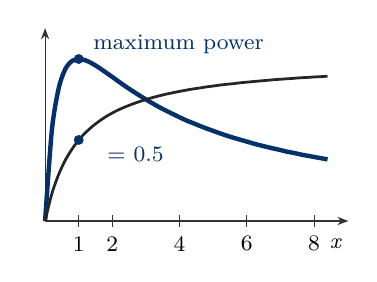
\begin{tikzpicture}[line join=round]
\draw[-{Stealth[length=4pt]},black!80] (0.720,-2.628) -- (4.572,-2.628);
\draw[-{Stealth[length=4pt]},black!80] (0.720,-2.628) -- (0.720,-0.180);
\draw[FAUblue,line width=1.6pt] plot[smooth,tension=0.5] coordinates {(0.720,-2.628) (0.805,-1.484) (0.891,-0.949) (0.976,-0.700) (1.062,-0.596) (1.147,-0.571) (1.232,-0.587) (1.318,-0.628) (1.403,-0.680) (1.489,-0.740) (1.574,-0.799) (1.659,-0.861) (1.745,-0.921) (1.830,-0.978) (1.916,-1.032) (2.001,-1.085) (2.086,-1.135) (2.172,-1.184) (2.257,-1.227) (2.343,-1.270) (2.428,-1.311) (2.513,-1.351) (2.599,-1.385) (2.684,-1.420) (2.769,-1.453) (2.855,-1.484) (2.940,-1.515) (3.026,-1.544) (3.111,-1.571) (3.196,-1.595) (3.282,-1.620) (3.367,-1.645) (3.453,-1.667) (3.538,-1.688) (3.623,-1.708) (3.709,-1.727) (3.794,-1.748) (3.880,-1.764) (3.965,-1.783) (4.050,-1.799) (4.136,-1.815) (4.221,-1.830) (4.307,-1.846)};
\draw[black!85,line width=1pt] plot[smooth,tension=0.5] coordinates {(0.720,-2.628) (0.805,-2.284) (0.891,-2.040) (0.976,-1.857) (1.062,-1.715) (1.147,-1.599) (1.232,-1.507) (1.318,-1.429) (1.403,-1.363) (1.489,-1.305) (1.574,-1.256) (1.659,-1.213) (1.745,-1.176) (1.830,-1.143) (1.916,-1.112) (2.001,-1.085) (2.086,-1.060) (2.172,-1.038) (2.257,-1.017) (2.343,-0.999) (2.428,-0.982) (2.513,-0.966) (2.599,-0.951) (2.684,-0.939) (2.769,-0.925) (2.855,-0.914) (2.940,-0.902) (3.026,-0.892) (3.111,-0.884) (3.196,-0.873) (3.282,-0.865) (3.367,-0.857) (3.453,-0.849) (3.538,-0.842) (3.623,-0.834) (3.709,-0.828) (3.794,-0.822) (3.880,-0.816) (3.965,-0.809) (4.050,-0.805) (4.136,-0.799) (4.221,-0.795) (4.307,-0.789)};
\fill[FAUblue] (1.147,-0.571) circle (0.063);
\node[anchor=west,text=FAUblue,fill=white,fill opacity=0.85,text opacity=1,inner sep=1pt,font=\footnotesize] at (1.291,-0.391) {maximum power};
\fill[FAUblue] (1.147,-1.599) circle (0.063);
\node[anchor=west,text=FAUblue,fill=white,fill opacity=0.85,text opacity=1,inner sep=1pt,font=\footnotesize] at (1.291,-1.779) {η = 0.5};
\node[anchor=east,inner sep=1pt,font=\footnotesize] at (4.536,-2.916) {\textit{x}};
\node[anchor=east,inner sep=1pt,font=\footnotesize] at (0.576,-0.288) {\textit{}};
\draw[black!80] (1.147,-2.556) -- (1.147,-2.700);
\node[,inner sep=1pt,font=\footnotesize] at (1.147,-2.916) {1};
\draw[black!80] (1.574,-2.556) -- (1.574,-2.700);
\node[,inner sep=1pt,font=\footnotesize] at (1.574,-2.916) {2};
\draw[black!80] (2.428,-2.556) -- (2.428,-2.700);
\node[,inner sep=1pt,font=\footnotesize] at (2.428,-2.916) {4};
\draw[black!80] (3.282,-2.556) -- (3.282,-2.700);
\node[,inner sep=1pt,font=\footnotesize] at (3.282,-2.916) {6};
\draw[black!80] (4.136,-2.556) -- (4.136,-2.700);
\node[,inner sep=1pt,font=\footnotesize] at (4.136,-2.916) {8};
\end{tikzpicture}\par\smallskip{\small\raggedright \textbf{Power and efficiency against the load.} \textit{x} is the load resistance as a multiple of \textit{R}\textsubscript{i}. The power ratio {\small\ensuremath{\dfrac{{P}_{\mathrm{L}}}{{P}_{\mathrm{L},\text{max}}}}} = {\small\ensuremath{\dfrac{4{x}}{(1\, +\, {x})^{2}}}} (blue) peaks at \textit{x} = 1; the efficiency \textit{η} = {\small\ensuremath{\dfrac{{x}}{1\, +\, {x}}}} (black) is only 0.5 there and keeps rising as the load grows.\par}\end{minipage}
\end{center}

\begin{workedbox}{Worked example \ensuremath{\cdot} matched versus efficient}
A source has \textit{U}\textsubscript{0} = 12 V and \textit{R}\textsubscript{i} = 2 Ω.

\Needspace{4\baselineskip}
\begin{enumerate}
\item Matched load \textit{R}\textsubscript{L} = 2 Ω: \textit{I} = 3 A, \textit{P}\textsubscript{L} = 3 A \ensuremath{\cdot} 3 A \ensuremath{\cdot} 2 Ω = 18 W = {\small\ensuremath{\dfrac{144}{8}}} W, \textit{P}\textsubscript{total} = 36 W, \textit{η} = 50 \%.
\item Load \textit{R}\textsubscript{L} = 8 Ω: \textit{I} = 1.2 A, \textit{P}\textsubscript{L} = 1.44 \ensuremath{\cdot} 8 W = 11.52 W, \textit{P}\textsubscript{total} = 14.4 W, \textit{η} = 80 \%.
\end{enumerate}

Check: the larger load gets less power but wastes far less. The power ratio {\small\ensuremath{\dfrac{11.52}{18}}} = 0.64 matches {\small\ensuremath{\dfrac{4\, \cdot \, 4}{(1\, +\, 4)^{2}}}} = 0.64 at \textit{x} = 4.
\end{workedbox}

\Needspace{7\baselineskip}
\begin{notebox}\textbf{Trap:} the divider formulas only hold when one current flows through the whole chain (voltage divider) or one voltage lies across all branches (current divider). Check that nothing branches off before you use them.\end{notebox}

\Needspace{6\baselineskip}
\begin{notebox}\textbf{Sign check:} current divider: the larger current goes through the smaller resistance. If your result says otherwise, the resistances are swapped in the formula.\end{notebox}

\Needspace{6\baselineskip}
\begin{notebox}\textbf{Memory hook:} maximum power is a compromise: half the voltage, half the short-circuit current, half the power lost.\end{notebox}

\Needspace{5\baselineskip}
\begin{notebox}\textbf{Near miss:} for \textit{R}\textsubscript{1} = 4 Ω, \textit{R}\textsubscript{2} = 6 Ω and \textit{R}\textsubscript{L} = 6 Ω, “\textit{U}\textsubscript{2} = {\small\ensuremath{\dfrac{6}{10}}}\textit{U}” uses the unloaded formula. The load halves the lower resistor to 3 Ω, so \textit{U}\textsubscript{2} = {\small\ensuremath{\dfrac{3}{7}}}\textit{U}.\end{notebox}

\Needspace{4\baselineskip}
\Needspace{9\baselineskip}
\begin{recallbox}{Recall check \ensuremath{\cdot} answer before opening}
\Needspace{5\baselineskip}
\begin{enumerate}
\item Three 30 Ω resistors are in parallel. What is the total?
\item Why does a load lower the tap voltage of a divider?
\item What is the efficiency at maximum power transfer?
\end{enumerate}

\nopagebreak[4]{\small\itshape Answers: see “3.5 Simple Resistor Networks” under Answers at the end.}
\end{recallbox}
\end{keepsection}
\end{keepsection}

\begin{keepsection}
\Needspace{14\baselineskip}
\section{3.6 Analysing More Extensive Networks}

\Needspace{11\baselineskip}
The shortcuts of §3.5 run out once a network has several sources or no clean series and parallel groups. Linearity gives one more shortcut, superposition, and node-voltage analysis gives a method that always works.

\begin{plainbox}\textbf{In plain words:} in a network of resistors and sources every equation is linear, so effects simply add. \textbf{Superposition} uses this: switch on one source at a time, solve, and add the partial answers. For a systematic solution, \textbf{node-voltage analysis} picks one node as zero potential and takes the other nodes’ potentials as the unknowns; every branch current is then a potential difference times a conductance, and KCL at each node gives the equations. The \textbf{Wheatstone bridge} is a classic network solved this way and used to measure resistances.\end{plainbox}

\begin{keepsection}
\Needspace{11\baselineskip}
\subsection{Superposition}

\begin{equationcard}{Superposition principle}
\[ \begin{gathered} {X}\, =\, {X}_{\mathrm{a}}\, +\, {X}_{\mathrm{b}}\, +\, … \\ \text{voltage}\, \text{source}\, \text{off}\, \to \, \text{short}\, \text{circuit} \\ \text{current}\, \text{source}\, \text{off}\, \to \, \text{open}\, \text{circuit} \end{gathered} \]
{\small \emph{Read it as: “the total response is the sum of the responses to each source alone”.}\par \textit{X} is any branch current or voltage; \textit{X}\textsubscript{a}, \textit{X}\textsubscript{b}, … are the values with only one source active. Internal resistances of real sources stay in place. Powers do not superpose: \textit{P} = \textit{R}\textit{I}\textsuperscript{2} is quadratic, so (\textit{I}\textsubscript{a} + \textit{I}\textsubscript{b})\textsuperscript{2} \ensuremath{\neq} \textit{I}\textsubscript{a}\textsuperscript{2} + \textit{I}\textsubscript{b}\textsuperscript{2}.}
\end{equationcard}

\begin{workedbox}{Worked example \ensuremath{\cdot} two sources and one resistor current}
\textit{U}\textsubscript{0} = 10 V with \textit{R}\textsubscript{1} = 2 Ω in series feeds a node; \textit{R}\textsubscript{2} = 3 Ω runs from that node to the return wire, and an ideal current source \textit{I}\textsubscript{0} = 1 A pushes current into the same node. Find the current \textit{I}\textsubscript{2} down through \textit{R}\textsubscript{2}.

\Needspace{9\baselineskip}
\begin{enumerate}
\item Only \textit{U}\textsubscript{0} on (current source open): \textit{R}\textsubscript{1} and \textit{R}\textsubscript{2} are in series, \textit{I}\textsubscript{2a} = {\small\ensuremath{\dfrac{10\, \mathrm{V}}{5\, Ω}}} = 2 A.
\item Only \textit{I}\textsubscript{0} on (voltage source shorted): \textit{R}\textsubscript{1} and \textit{R}\textsubscript{2} are in parallel across the current source; the current divider gives \textit{I}\textsubscript{2b} = 1 A \ensuremath{\cdot} {\small\ensuremath{\dfrac{2\, Ω}{5\, Ω}}} = 0.4 A.
\item Add: \textit{I}\textsubscript{2} = 2 A + 0.4 A = 2.4 A, so \textit{R}\textsubscript{2} takes 2.4\textsuperscript{2} \ensuremath{\cdot} 3 W = 17.28 W.
\item Adding the partial powers instead would give 12 W + 0.48 W = 12.48 W, which is wrong by the cross term 2 \ensuremath{\cdot} 2 A \ensuremath{\cdot} 0.4 A \ensuremath{\cdot} 3 Ω = 4.8 W.
\end{enumerate}

Check with KCL at the node: the current in \textit{R}\textsubscript{1} is (10 V \ensuremath{-} 7.2 V) ÷ 2 Ω = 1.4 A, plus 1 A from the source, gives 2.4 A into \textit{R}\textsubscript{2}, and 2.4 A \ensuremath{\cdot} 3 Ω = 7.2 V.
\end{workedbox}
\end{keepsection}

\begin{keepsection}
\Needspace{10\baselineskip}
\subsection{How many unknowns}

Each branch has one current and one voltage, but its current–voltage rule ties them together, so every branch carries only one unknown: for a resistor either \textit{U} or \textit{I} (the other follows from Ohm’s law); for an ideal voltage source the current; for an ideal current source the voltage. A network with \textit{N}\textsubscript{b} branches has at most \textit{N}\textsubscript{b} unknowns. Each method of this section keeps some of them as unknowns (node-voltage analysis keeps only node potentials) and produces one independent linear equation per unknown it keeps.
\end{keepsection}

\begin{keepsection}
\Needspace{18\baselineskip}
\subsection{Node-voltage analysis}

\Needspace{15\baselineskip}
\begin{enumerate}
\item Choose a reference node n\textsubscript{0} with φ\textsubscript{0} = 0.
\item Number the other nodes n\textsubscript{1}, …, n\textsubscript{\textit{N}\textsubscript{n} \ensuremath{-} 1}.
\item Enclose nodes joined by an ideal voltage source: their potentials differ by the known source voltage, so the enclosure counts as one node.
\item Give each node, or each enclosure, one unknown potential φ.
\item Give every branch a current with a reference arrow.
\item Write KCL for every node and enclosure, with each resistor current written as a potential difference times a conductance and each current-source current inserted as given. Drop one equation: it is linearly dependent on the rest.
\item Solve the linear system (Gaussian elimination or Cramer’s rule, Appendix B.7) and compute the wanted currents and voltages.
\end{enumerate}

\begin{equationcard}{Branch current from two potentials}
\[ \begin{gathered} {I}_{{k}}\, =\, \dfrac{φ_{{x}}\, -\, φ_{{y}}}{{R}_{{k}}}\, =\, (φ_{{x}}\, -\, φ_{{y}}){G}_{{k}} \end{gathered} \]
{\small \emph{Read it as: “the current from x to y is the potential difference times the conductance”.}\par The arrow of the current points from node \textit{x} to node \textit{y} through the resistor (load convention). Arranged by unknowns, each node equation has the sum of the conductances at that node as the coefficient of its own potential and minus the conductance to each neighbour as the other coefficients. (That pattern follows directly from the notes’ worked equations; the notes do not state it as a rule.)}
\end{equationcard}

\Needspace{14\baselineskip}
\begin{center}
\begin{minipage}[t]{0.950\linewidth}\centering
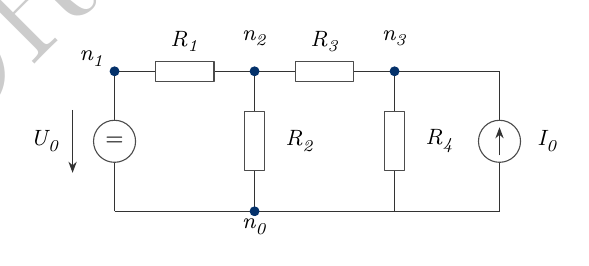
\begin{tikzpicture}[line join=round]
\draw[black!80] (1.765,-2.921) -- (1.765,-1.143);
\draw[black!80] (1.765,-1.143) -- (5.321,-1.143);
\draw[black!80] (5.321,-1.143) -- (6.654,-1.143);
\draw[black!80] (6.654,-1.143) -- (6.654,-2.921);
\draw[black!80] (1.765,-2.921) -- (6.654,-2.921);
\draw[black!80] (3.543,-1.143) -- (3.543,-2.921);
\draw[black!80] (5.321,-1.143) -- (5.321,-2.921);
\draw[draw=black!70,fill=white] (1.765,-2.032) circle (0.267);
\node[fill=white,fill opacity=0.85,text opacity=1,inner sep=1pt,font=\footnotesize] at (1.765,-2.032) {=};
\filldraw[draw=black!70,fill=white] (2.281,-1.268) rectangle (3.028,-1.019);
\filldraw[draw=black!70,fill=white] (3.419,-2.405) rectangle (3.668,-1.659);
\filldraw[draw=black!70,fill=white] (4.059,-1.268) rectangle (4.805,-1.019);
\filldraw[draw=black!70,fill=white] (5.196,-2.405) rectangle (5.445,-1.659);
\draw[draw=black!70,fill=white] (6.654,-2.032) circle (0.267);
\draw[-{Stealth[length=4pt]},black!80] (6.654,-2.210) -- (6.654,-1.854);
\fill[FAUblue] (1.765,-1.143) circle (0.063);
\fill[FAUblue] (3.543,-1.143) circle (0.063);
\fill[FAUblue] (5.321,-1.143) circle (0.063);
\fill[FAUblue] (3.543,-2.921) circle (0.063);
\draw[-{Stealth[length=4pt]},black!80] (1.232,-1.632) -- (1.232,-2.432);
\node[anchor=east,fill=white,fill opacity=0.85,text opacity=1,inner sep=1pt,font=\footnotesize] at (1.106,-2.032) {\textit{U\textsubscript{0}}};
\node[fill=white,fill opacity=0.85,text opacity=1,inner sep=1pt,font=\footnotesize] at (2.654,-0.767) {\textit{R\textsubscript{1}}};
\node[fill=white,fill opacity=0.85,text opacity=1,inner sep=1pt,font=\footnotesize] at (4.432,-0.767) {\textit{R\textsubscript{3}}};
\node[anchor=west,fill=white,fill opacity=0.85,text opacity=1,inner sep=1pt,font=\footnotesize] at (3.891,-2.032) {\textit{R\textsubscript{2}}};
\node[anchor=west,fill=white,fill opacity=0.85,text opacity=1,inner sep=1pt,font=\footnotesize] at (5.669,-2.032) {\textit{R\textsubscript{4}}};
\node[anchor=west,fill=white,fill opacity=0.85,text opacity=1,inner sep=1pt,font=\footnotesize] at (7.091,-2.032) {\textit{I\textsubscript{0}}};
\node[anchor=east,fill=white,fill opacity=0.85,text opacity=1,inner sep=1pt,font=\footnotesize] at (1.675,-0.981) {\textit{n\textsubscript{1}}};
\node[fill=white,fill opacity=0.85,text opacity=1,inner sep=1pt,font=\footnotesize] at (3.543,-0.723) {\textit{n\textsubscript{2}}};
\node[fill=white,fill opacity=0.85,text opacity=1,inner sep=1pt,font=\footnotesize] at (5.321,-0.723) {\textit{n\textsubscript{3}}};
\node[fill=white,fill opacity=0.85,text opacity=1,inner sep=1pt,font=\footnotesize] at (3.543,-3.119) {\textit{n\textsubscript{0}}};
\end{tikzpicture}\par\smallskip{\small\raggedright \textbf{The node-voltage example.} Reference node n\textsubscript{0} along the bottom. The ideal source fixes φ\textsubscript{1} = \textit{U}\textsubscript{0}, so only φ\textsubscript{2} and φ\textsubscript{3} are unknown. The current source \textit{I}\textsubscript{0} pushes current up into n\textsubscript{3}.\par}\end{minipage}
\end{center}

\begin{workedbox}{Worked example \ensuremath{\cdot} two unknown potentials}
\textit{U}\textsubscript{0} = 10 V, \textit{R}\textsubscript{1} = 2 Ω, \textit{R}\textsubscript{2} = 4 Ω, \textit{R}\textsubscript{3} = 2 Ω, \textit{R}\textsubscript{4} = 5 Ω and \textit{I}\textsubscript{0} = 0.5 A, connected as in the figure.

\Needspace{11\baselineskip}
\begin{enumerate}
\item Steps 1–4: n\textsubscript{0} is the reference; the source encloses n\textsubscript{0} and n\textsubscript{1}, so φ\textsubscript{1} = 10 V; the unknowns are φ\textsubscript{2} and φ\textsubscript{3}.
\item KCL at n\textsubscript{2} (inflow positive): {\small\ensuremath{\dfrac{10\, \mathrm{V}\, -\, φ_{2}}{2\, Ω}}} \ensuremath{-} {\small\ensuremath{\dfrac{φ_{2}}{4\, Ω}}} \ensuremath{-} {\small\ensuremath{\dfrac{φ_{2}\, -\, φ_{3}}{2\, Ω}}} = 0, that is 1.25 S \ensuremath{\cdot} φ\textsubscript{2} \ensuremath{-} 0.5 S \ensuremath{\cdot} φ\textsubscript{3} = 5 A.
\item KCL at n\textsubscript{3}: {\small\ensuremath{\dfrac{φ_{2}\, -\, φ_{3}}{2\, Ω}}} \ensuremath{-} {\small\ensuremath{\dfrac{φ_{3}}{5\, Ω}}} + 0.5 A = 0, that is \ensuremath{-}0.5 S \ensuremath{\cdot} φ\textsubscript{2} + 0.7 S \ensuremath{\cdot} φ\textsubscript{3} = 0.5 A.
\item Cramer: the determinant is 1.25 \ensuremath{\cdot} 0.7 \ensuremath{-} 0.25 = 0.625, so φ\textsubscript{2} = {\small\ensuremath{\dfrac{5\, \cdot \, 0.7\, +\, 0.5\, \cdot \, 0.5}{0.625}}} V = 6 V and φ\textsubscript{3} = {\small\ensuremath{\dfrac{1.25\, \cdot \, 0.5\, +\, 0.5\, \cdot \, 5}{0.625}}} V = 5 V.
\item Currents: \textit{R}\textsubscript{1} carries 2 A, \textit{R}\textsubscript{2} 1.5 A, \textit{R}\textsubscript{3} 0.5 A and \textit{R}\textsubscript{4} 1 A.
\end{enumerate}

Check the power balance: the resistors take 8 + 9 + 0.5 + 5 = 22.5 W; the voltage source delivers 10 V \ensuremath{\cdot} 2 A = 20 W and the current source 5 V \ensuremath{\cdot} 0.5 A = 2.5 W, together 22.5 W.
\end{workedbox}
\end{keepsection}

\begin{keepsection}
\Needspace{12\baselineskip}
\subsection{The Wheatstone bridge}

\begin{equationcard}{Diagonal voltage and balance condition}
\[ \begin{gathered} {U}_{\mathrm{D}}\, =\, \dfrac{{G}_{{x}}{G}_{4}\, -\, {G}_{2}{G}_{3}}{({G}_{{x}}\, +\, {G}_{2}\, +\, {G}_{\mathrm{i}})({G}_{3}\, +\, {G}_{4}\, +\, {G}_{\mathrm{i}})\, -\, {G}_{\mathrm{i}}^{2}}\, {U}_{0} \\ {U}_{\mathrm{D}}\, =\, 0\, \Leftrightarrow \, {R}_{{x}}{R}_{4}\, =\, {R}_{2}{R}_{3}\, \Leftrightarrow \, \dfrac{{R}_{{x}}}{{R}_{2}}\, =\, \dfrac{{R}_{3}}{{R}_{4}} \end{gathered} \]
{\small \emph{Read it as: “the bridge is balanced when R x times R four equals R two times R three”.}\par The first line comes from node-voltage analysis with φ\textsubscript{2} and φ\textsubscript{3} unknown (derivation below). In practice one known resistor (here \textit{R}\textsubscript{2}) is adjusted until the meter reads zero; then both sides are unloaded dividers with equal ratios. At balance no current flows through the meter, so its finite \textit{R}\textsubscript{i} does not falsify the result.}
\end{equationcard}
\end{keepsection}

\begin{keepsection}
\Needspace{13\baselineskip}
\subsection{Derivation: the diagonal voltage}

\Needspace{10\baselineskip}
\begin{enumerate}
\item Reference n\textsubscript{0} at the bottom; the source fixes φ\textsubscript{1} = \textit{U}\textsubscript{0}; unknowns φ\textsubscript{2} (left tap) and φ\textsubscript{3} (right tap); the meter is a conductance \textit{G}\textsubscript{i} between the taps.
\item KCL at n\textsubscript{2}: (\textit{U}\textsubscript{0} \ensuremath{-} φ\textsubscript{2})\textit{G}\textsubscript{\textit{x}} \ensuremath{-} φ\textsubscript{2}\textit{G}\textsubscript{2} \ensuremath{-} (φ\textsubscript{2} \ensuremath{-} φ\textsubscript{3})\textit{G}\textsubscript{i} = 0. At n\textsubscript{3}: (\textit{U}\textsubscript{0} \ensuremath{-} φ\textsubscript{3})\textit{G}\textsubscript{3} \ensuremath{-} φ\textsubscript{3}\textit{G}\textsubscript{4} + (φ\textsubscript{2} \ensuremath{-} φ\textsubscript{3})\textit{G}\textsubscript{i} = 0.
\item Sorted: (\textit{G}\textsubscript{\textit{x}} + \textit{G}\textsubscript{2} + \textit{G}\textsubscript{i})φ\textsubscript{2} \ensuremath{-} \textit{G}\textsubscript{i}φ\textsubscript{3} = \textit{U}\textsubscript{0}\textit{G}\textsubscript{\textit{x}} and \ensuremath{-}\textit{G}\textsubscript{i}φ\textsubscript{2} + (\textit{G}\textsubscript{3} + \textit{G}\textsubscript{4} + \textit{G}\textsubscript{i})φ\textsubscript{3} = \textit{U}\textsubscript{0}\textit{G}\textsubscript{3}.
\item Cramer’s rule gives φ\textsubscript{2} and φ\textsubscript{3} over the same determinant \textit{D}; in \textit{U}\textsubscript{D} = φ\textsubscript{2} \ensuremath{-} φ\textsubscript{3} the terms \textit{G}\textsubscript{\textit{x}}\textit{G}\textsubscript{3}, \textit{G}\textsubscript{\textit{x}}\textit{G}\textsubscript{i} and \textit{G}\textsubscript{3}\textit{G}\textsubscript{i} cancel, leaving \textit{U}\textsubscript{D} = {\small\ensuremath{\dfrac{{G}_{{x}}{G}_{4}\, -\, {G}_{2}{G}_{3}}{{D}}}} \textit{U}\textsubscript{0}.
\item \textit{U}\textsubscript{D} = 0 exactly when \textit{G}\textsubscript{\textit{x}}\textit{G}\textsubscript{4} = \textit{G}\textsubscript{2}\textit{G}\textsubscript{3}, that is \textit{R}\textsubscript{\textit{x}}\textit{R}\textsubscript{4} = \textit{R}\textsubscript{2}\textit{R}\textsubscript{3}.
\end{enumerate}

\Needspace{14\baselineskip}
\begin{center}
\begin{minipage}[t]{0.950\linewidth}\centering
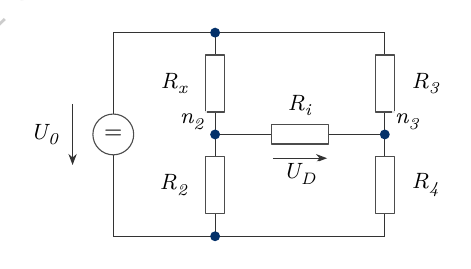
\begin{tikzpicture}[line join=round]
\draw[black!80] (1.725,-3.449) -- (1.725,-0.863);
\draw[black!80] (1.725,-0.863) -- (5.173,-0.863);
\draw[black!80] (1.725,-3.449) -- (5.173,-3.449);
\draw[black!80] (3.018,-0.863) -- (3.018,-3.449);
\draw[black!80] (5.173,-0.863) -- (5.173,-3.449);
\draw[black!80] (3.018,-2.156) -- (5.173,-2.156);
\draw[draw=black!70,fill=white] (1.725,-2.156) circle (0.259);
\node[fill=white,fill opacity=0.85,text opacity=1,inner sep=1pt,font=\footnotesize] at (1.725,-2.156) {=};
\filldraw[draw=black!70,fill=white] (2.897,-1.871) rectangle (3.139,-1.147);
\filldraw[draw=black!70,fill=white] (2.897,-3.164) rectangle (3.139,-2.440);
\filldraw[draw=black!70,fill=white] (5.052,-1.871) rectangle (5.294,-1.147);
\filldraw[draw=black!70,fill=white] (5.052,-3.164) rectangle (5.294,-2.440);
\filldraw[draw=black!70,fill=white] (3.733,-2.277) rectangle (4.457,-2.035);
\fill[FAUblue] (3.018,-0.863) circle (0.063);
\fill[FAUblue] (3.018,-3.449) circle (0.063);
\fill[FAUblue] (3.018,-2.156) circle (0.063);
\fill[FAUblue] (5.173,-2.156) circle (0.063);
\draw[-{Stealth[length=4pt]},black!80] (1.208,-1.768) -- (1.208,-2.544);
\node[anchor=east,fill=white,fill opacity=0.85,text opacity=1,inner sep=1pt,font=\footnotesize] at (1.082,-2.156) {\textit{U\textsubscript{0}}};
\node[anchor=east,fill=white,fill opacity=0.85,text opacity=1,inner sep=1pt,font=\footnotesize] at (2.720,-1.509) {\textit{R\textsubscript{x}}};
\node[anchor=east,fill=white,fill opacity=0.85,text opacity=1,inner sep=1pt,font=\footnotesize] at (2.720,-2.802) {\textit{R\textsubscript{2}}};
\node[anchor=west,fill=white,fill opacity=0.85,text opacity=1,inner sep=1pt,font=\footnotesize] at (5.471,-1.509) {\textit{R\textsubscript{3}}};
\node[anchor=west,fill=white,fill opacity=0.85,text opacity=1,inner sep=1pt,font=\footnotesize] at (5.471,-2.802) {\textit{R\textsubscript{4}}};
\node[fill=white,fill opacity=0.85,text opacity=1,inner sep=1pt,font=\footnotesize] at (4.095,-1.786) {\textit{R\textsubscript{i}}};
\draw[-{Stealth[length=4pt]},black!80] (3.751,-2.458) -- (4.440,-2.458);
\node[fill=white,fill opacity=0.85,text opacity=1,inner sep=1pt,font=\footnotesize] at (4.095,-2.656) {\textit{U\textsubscript{D}}};
\node[anchor=east,fill=white,fill opacity=0.85,text opacity=1,inner sep=1pt,font=\footnotesize] at (2.928,-1.994) {\textit{n\textsubscript{2}}};
\node[anchor=west,fill=white,fill opacity=0.85,text opacity=1,inner sep=1pt,font=\footnotesize] at (5.263,-1.994) {\textit{n\textsubscript{3}}};
\end{tikzpicture}\par\smallskip{\small\raggedright \textbf{A Wheatstone bridge.} Two voltage dividers share the source: \textit{R}\textsubscript{\textit{x}} over \textit{R}\textsubscript{2} on the left and \textit{R}\textsubscript{3} over \textit{R}\textsubscript{4} on the right. A voltmeter with internal resistance \textit{R}\textsubscript{i} measures the diagonal voltage \textit{U}\textsubscript{D} between the taps n\textsubscript{2} and n\textsubscript{3}.\par}\end{minipage}
\end{center}

\begin{workedbox}{Worked example \ensuremath{\cdot} finding an unknown resistance}
A bridge has \textit{R}\textsubscript{3} = 470 Ω and \textit{R}\textsubscript{4} = 1 kΩ. The meter reads zero when \textit{R}\textsubscript{2} = 100 Ω.

\Needspace{5\baselineskip}
\begin{enumerate}
\item Balance: \textit{R}\textsubscript{\textit{x}} = {\small\ensuremath{\dfrac{{R}_{2}{R}_{3}}{{R}_{4}}}} = {\small\ensuremath{\dfrac{100\, Ω\, \cdot \, 470\, Ω}{1000\, Ω}}} = 47 Ω.
\item Check the dividers with \textit{U}\textsubscript{0} = 10 V: left tap 10 V \ensuremath{\cdot} {\small\ensuremath{\dfrac{100}{147}}} \ensuremath{\approx} 6.80 V, right tap 10 V \ensuremath{\cdot} {\small\ensuremath{\dfrac{1000}{1470}}} \ensuremath{\approx} 6.80 V.
\end{enumerate}

Check: equal tap potentials, so \textit{U}\textsubscript{D} = 0 and the meter current is zero, whatever its \textit{R}\textsubscript{i}.
\end{workedbox}

\Needspace{7\baselineskip}
\begin{notebox}\textbf{Trap:} switching off a voltage source means replacing it with a wire, not removing it. Removing it would leave an open circuit and change the network.\end{notebox}

\Needspace{7\baselineskip}
\begin{notebox}\textbf{Sign check:} in each node equation the coefficient of the node’s own potential is positive (the sum of its conductances) and every neighbour’s coefficient is negative. A sign that breaks this pattern points to a wrong current arrow.\end{notebox}

\Needspace{7\baselineskip}
\begin{notebox}\textbf{Memory hook:} superposition: voltage source off = short, current source off = open; add currents and voltages, never powers.\end{notebox}

\Needspace{6\baselineskip}
\begin{notebox}\textbf{Near miss:} in the superposition example, keeping the 10 V source while computing the 1 A part gives a “partial” current that already contains the first part, so the sum counts it twice. Every source except one must be off in each step.\end{notebox}

\Needspace{11\baselineskip}
\begin{recallbox}{Recall check \ensuremath{\cdot} answer before opening}
\Needspace{6\baselineskip}
\begin{enumerate}
\item A network has 5 nodes and one ideal voltage source between two of them, neither the reference. How many unknown potentials are there?
\item Why can partial powers not be added?
\item What is the balance condition of a Wheatstone bridge?
\end{enumerate}

\nopagebreak[4]{\small\itshape Answers: see “3.6 Analysing More Extensive Networks” under Answers at the end.}
\end{recallbox}
\end{keepsection}
\end{keepsection}

\begin{keepsection}
\Needspace{32\baselineskip}
\section{Formula map and units}

\Needspace{32\baselineskip}
Units are SI: voltage in V, current in A, resistance in Ω, conductance in S and power in W.

\Needspace{10\baselineskip}
\begin{center}\small\begin{tabularx}{\linewidth}{>{\raggedright\arraybackslash}X>{\raggedright\arraybackslash}X>{\raggedright\arraybackslash}X>{\raggedright\arraybackslash}X}\toprule
\textbf{Topic} & \textbf{Relation} & \textbf{Unit} & \textbf{Check} \\ \midrule
Conductance & \textit{G} = {\small\ensuremath{\dfrac{1}{{R}}}} & S = Ω\textsuperscript{\ensuremath{-}1} & \textit{R} \ensuremath{>} 0 for every resistor. \\
Real voltage source & \textit{U} = \textit{U}\textsubscript{0} \ensuremath{-} \textit{I}\textit{R}\textsubscript{i}, \textit{I}\textsubscript{0} = {\small\ensuremath{\dfrac{{U}_{0}}{{R}_{\mathrm{i}}}}} & V, A, Ω & \textit{U} \ensuremath{\leq} \textit{U}\textsubscript{0} while delivering current. \\
Real current source & \textit{I} = \textit{I}\textsubscript{0} \ensuremath{-} {\small\ensuremath{\dfrac{{U}}{{R}_{\mathrm{i}}}}}, \textit{U}\textsubscript{0} = \textit{I}\textsubscript{0}\textit{R}\textsubscript{i} & A, V, Ω & Open-circuit voltage \textit{I}\textsubscript{0}\textit{R}\textsubscript{i}. \\
Source transformation & \textit{U}\textsubscript{0} = \textit{I}\textsubscript{0}\textit{R}\textsubscript{i}, same \textit{R}\textsubscript{i} & V = A \ensuremath{\cdot} Ω & Same terminal line; internal losses differ. \\
Dependent sources & α\textit{U}\textsubscript{cg}, β\textit{U}\textsubscript{cg}, γ\textit{I}\textsubscript{cg}, δ\textit{I}\textsubscript{cg} & α, δ: 1; β: S; γ: Ω & Output unit must match V or A. \\
Load convention & \textit{P} = \textit{U}\textit{I} absorbed & W & Negative: the part delivers power. \\
KVL & \ensuremath{\textstyle\sum} \textit{U}\textsubscript{μ} = 0 round a mesh & V & Arrow along travel +, against \ensuremath{-}. \\
KCL & \ensuremath{\textstyle\sum} \textit{I}\textsubscript{μ} = 0 at a node & A & One node equation is redundant. \\
Series, parallel & \textit{R}\textsubscript{total} = \ensuremath{\textstyle\sum} \textit{R}\textsubscript{\textit{n}}; \textit{G}\textsubscript{total} = \ensuremath{\textstyle\sum} \textit{G}\textsubscript{\textit{n}} & Ω; S & Series above the largest, parallel below the smallest. \\
Voltage divider & {\small\ensuremath{\dfrac{{U}_{{n}}}{{U}_{\text{total}}}}} = {\small\ensuremath{\dfrac{{R}_{{n}}}{{R}_{\text{total}}}}}; loaded: replace \textit{R}\textsubscript{2} by \textit{R}\textsubscript{2} \ensuremath{\parallel} \textit{R}\textsubscript{L} & 1 & Ratio between 0 and 1. \\
Current divider & {\small\ensuremath{\dfrac{{I}_{{n}}}{{I}_{\text{total}}}}} = {\small\ensuremath{\dfrac{{G}_{{n}}}{{G}_{\text{total}}}}}; {\small\ensuremath{\dfrac{{I}_{2}}{{I}}}} = {\small\ensuremath{\dfrac{{R}_{1}}{{R}_{1}\, +\, {R}_{2}}}} & 1 & Larger current through the smaller resistance. \\
Load power & \textit{P}\textsubscript{L} = \textit{U}\textsubscript{0}\textsuperscript{2}{\small\ensuremath{\dfrac{{R}_{\mathrm{L}}}{({R}_{\mathrm{i}}\, +\, {R}_{\mathrm{L}})^{2}}}} & W & 0 at open and short circuit. \\
Maximum power & \textit{R}\textsubscript{L} = \textit{R}\textsubscript{i}, \textit{P}\textsubscript{L,max} = {\small\ensuremath{\dfrac{{U}_{0}^{2}}{4{R}_{\mathrm{i}}}}} & W & Efficiency 50 \% there. \\
Efficiency & \textit{η} = {\small\ensuremath{\dfrac{{R}_{\mathrm{L}}}{{R}_{\mathrm{i}}\, +\, {R}_{\mathrm{L}}}}} & 1 & Between 0 and 1; near 1 needs \textit{R}\textsubscript{L} \ensuremath{\gg} \textit{R}\textsubscript{i}. \\
Node equation & \textit{I} = (φ\textsubscript{\textit{x}} \ensuremath{-} φ\textsubscript{\textit{y}})\textit{G} & A = V \ensuremath{\cdot} S & Own coefficient +, neighbours \ensuremath{-}. \\
Wheatstone balance & \textit{R}\textsubscript{\textit{x}}\textit{R}\textsubscript{4} = \textit{R}\textsubscript{2}\textit{R}\textsubscript{3} & Ω\textsuperscript{2} & Meter current zero at balance. \\
\bottomrule\end{tabularx}\end{center}
\end{keepsection}

\begin{keepsection}
\Needspace{9\baselineskip}
\section{Derive it cold}

\Needspace{6\baselineskip}
Rebuild these on blank paper before opening the derivations in the relevant sections.

\begin{enumerate}
\item Derive KVL from $\oint $ \textit{E} \ensuremath{\cdot} d\textit{s} = 0 by splitting the loop at its nodes. \hfill{\small\color{FAUblue}§3.4}
\item Derive KCL from $\oiint $ \textit{J} \ensuremath{\cdot} d\textit{A} = 0 for stationary currents. \hfill{\small\color{FAUblue}§3.4}
\item Show that real voltage and current sources are equivalent when \textit{U}\textsubscript{0} = \textit{I}\textsubscript{0}\textit{R}\textsubscript{i}, by deriving both terminal lines. \hfill{\small\color{FAUblue}§3.2}
\item Derive \textit{R}\textsubscript{total} = \ensuremath{\textstyle\sum} \textit{R}\textsubscript{\textit{n}} for series and \textit{G}\textsubscript{total} = \ensuremath{\textstyle\sum} \textit{G}\textsubscript{\textit{n}} for parallel resistors from KVL, KCL and Ohm’s law. \hfill{\small\color{FAUblue}§3.5}
\item Derive the unloaded voltage divider and current divider rules for two resistors. \hfill{\small\color{FAUblue}§3.5}
\item Derive the loaded voltage divider ratio {\small\ensuremath{\dfrac{{U}_{2}}{{U}}}} and show its limit for \textit{R}\textsubscript{L} \ensuremath{\to} \ensuremath{\infty}. \hfill{\small\color{FAUblue}§3.5}
\item Derive \textit{P}\textsubscript{L}(\textit{R}\textsubscript{L}), find its maximum at \textit{R}\textsubscript{L} = \textit{R}\textsubscript{i} and the value \textit{P}\textsubscript{L,max} = {\small\ensuremath{\dfrac{{U}_{0}^{2}}{4{R}_{\mathrm{i}}}}}. \hfill{\small\color{FAUblue}§3.5}
\item Derive the efficiency \textit{η} = {\small\ensuremath{\dfrac{{R}_{\mathrm{L}}}{{R}_{\mathrm{i}}\, +\, {R}_{\mathrm{L}}}}} and its value at maximum power. \hfill{\small\color{FAUblue}§3.5}
\item Set up the node equations of the Wheatstone bridge and derive the balance condition. \hfill{\small\color{FAUblue}§3.6}
\end{enumerate}
\end{keepsection}

\begin{keepsection}
\Needspace{21\baselineskip}
\section{Explain it}

\Needspace{18\baselineskip}
Answer aloud in complete sentences. Then compare with the model answer. (Retrieval and explanatory questioning [MIS, AMN, NEW].)

\Needspace{15\baselineskip}
\begin{enumerate}
\item \textbf{Why} may an ideal voltage source not be short-circuited, and an ideal current source not be left open?
\item \textbf{Why} do the two equivalent real sources behave differently inside even though no load can tell them apart?
\item \textbf{Why} does KVL hold for a mesh that is not a closed chain of wires?
\item \textbf{When} can you use the voltage-divider formula?
\item \textbf{Why} is maximum power transfer not what a power station wants?
\item \textbf{Why} can superposition add currents but not powers?
\item \textbf{Why} does node-voltage analysis drop one KCL equation?
\item \textbf{Why} does the balanced Wheatstone bridge give a correct result with a non-ideal voltmeter?
\end{enumerate}

\nopagebreak[4]{\small\itshape Answers: see “Explain it” under Answers at the end.}
\end{keepsection}

\clearpage

\begin{keepsection}
\Needspace{11\baselineskip}
\section{Mixed practice}

\Needspace{8\baselineskip}
Try all 24 problems before opening the answer key. The topics are interleaved, so identify the method before calculating. Round to three significant figures. (Desirable difficulty and varied retrieval [MIS, AMN].)

\begin{enumerate}
\item Find the total resistance of 10 Ω, 20 Ω and 30 Ω in parallel.
\item A real voltage source with \textit{U}\textsubscript{0} = 9 V and \textit{R}\textsubscript{i} = 1.5 Ω feeds a 3 Ω load. Find the current, the terminal voltage and the short-circuit current.
\item Four wires meet at a node. Wire 1 carries 4 A in, wire 2 carries 2.5 A out, and wire 3 carries \ensuremath{-}0.7 A with its arrow pointing out. Wire 4’s arrow points out. Find its current.
\item Two sources each drive a partial current through a 5 Ω resistor, 1 A and 2 A in the same direction. Find the resistor’s power, and the wrong answer that adding partial powers would give.
\item A part is measured with the load convention: \textit{U} = \ensuremath{-}4 V and \textit{I} = 2.5 A. Does it absorb or deliver power, and how much?
\item A divider of \textit{R}\textsubscript{1} = 3 kΩ and \textit{R}\textsubscript{2} = 9 kΩ is connected to 24 V. Find both partial voltages, unloaded.
\item Turn a real current source of \textit{I}\textsubscript{0} = 50 mA in parallel with \textit{R}\textsubscript{i} = 200 Ω into a real voltage source.
\item Find the conductance of a 250 Ω resistor and the current it draws at 5 V.
\item A source \textit{U}\textsubscript{0} = 12 V feeds node n\textsubscript{2} through \textit{R}\textsubscript{1} = 4 Ω; \textit{R}\textsubscript{2} = 12 Ω runs from n\textsubscript{2} to the reference node, and a 0.5 A current source pushes current into n\textsubscript{2}. Find φ\textsubscript{2}.
\item A 15 V source drives a single mesh with three resistors. Two resistor voltages, both pointing along the current, are 4 V and 6 V. Find the third.
\item A divider of \textit{R}\textsubscript{1} = \textit{R}\textsubscript{2} = 1 kΩ sits on 10 V. Find \textit{U}\textsubscript{2} with a load of 1 kΩ and with a load of 100 kΩ.
\item A source has \textit{U}\textsubscript{0} = 6 V and \textit{R}\textsubscript{i} = 3 Ω. Which load takes the most power, how much, and at what efficiency?
\item A current-controlled voltage source has γ = 200 Ω and a control current of 15 mA. Find its output voltage and say what happens if the control current reverses.
\item A Wheatstone bridge balances with \textit{R}\textsubscript{2} = 150 Ω, \textit{R}\textsubscript{3} = 220 Ω and \textit{R}\textsubscript{4} = 330 Ω. Find \textit{R}\textsubscript{\textit{x}}.
\item An ideal voltage source and three resistors are all connected between the same two wires. How many nodes and branches does the graph have?
\item A meter with internal resistance 10 Ω reads up to 1 mA. Which shunt extends it to 100 mA?
\item A closed box has three wires. 2 A flows in on the first and 5 A out on the second. What flows on the third?
\item You apply superposition to a network with a real voltage source (with internal resistance) and an ideal current source. What do you put in place of each source when it is switched off?
\item A source has \textit{R}\textsubscript{i} = 0.1 Ω. How large must the load be for an efficiency of at least 95 \%?
\item An ideal current source of 2 mA feeds a 4.7 kΩ resistor. Find the voltage. What happens to the voltage if the resistance is doubled?
\item A network has 5 nodes. An ideal voltage source joins two non-reference nodes. How many node equations do you solve?
\item A current of 60 mA divides between 2 kΩ and 3 kΩ in parallel. Find both branch currents.
\item A 3 A ideal current source drives a single loop through an 8 Ω resistor and a 6 V ideal voltage source, entering the voltage source at its + terminal. What voltage does the current source produce?
\item A four-terminal network carries 3 mA in at terminal 1, 3 mA out at 1\ensuremath{{}^{\prime}}, 2 mA in at 2 and 2 mA out at 2\ensuremath{{}^{\prime}}. Is it a two-port? What if instead 2.5 mA leaves at 1\ensuremath{{}^{\prime}} and 2.5 mA at 2\ensuremath{{}^{\prime}}?
\end{enumerate}

\nopagebreak[4]{\small\itshape Answers: see “Mixed practice” under Answers at the end.}
\end{keepsection}

\begin{keepsection}
\Needspace{6\baselineskip}
\section{Exam-style problems}

Allow about 20 minutes for each. Work every part before checking the answer. Afterward, note where you lost a step and revisit the cited sections.

\begin{keepsection}
\Needspace{14\baselineskip}
\subsection{1 \ensuremath{\cdot} A battery, a loaded divider and the best load}

\Needspace{11\baselineskip}
A battery with \textit{U}\textsubscript{0} = 12 V and \textit{R}\textsubscript{i} = 1 Ω feeds a divider of \textit{R}\textsubscript{1} = 5 Ω on top and \textit{R}\textsubscript{2} = 6 Ω below. A load \textit{R}\textsubscript{L} = 3 Ω is connected across \textit{R}\textsubscript{2}.

\Needspace{8\baselineskip}
\begin{enumerate}
\item Find the battery current, the battery’s terminal voltage and the load voltage.
\item Find the currents in \textit{R}\textsubscript{2} and \textit{R}\textsubscript{L} and check them with KCL.
\item Find the efficiency: the power in \textit{R}\textsubscript{L} as a share of the power the ideal source supplies.
\item Replace everything to the left of \textit{R}\textsubscript{L} by one real voltage source, using source transformations, and find the load that would take the most power. Compare with 3 Ω.
\end{enumerate}

\nopagebreak[4]{\small\itshape Answers: see “Exam-style problems” under Answers at the end.}
\end{keepsection}

\begin{keepsection}
\Needspace{13\baselineskip}
\subsection{2 \ensuremath{\cdot} Node voltage, superposition and a power balance}

\Needspace{10\baselineskip}
A source \textit{U}\textsubscript{0} = 12 V feeds node n\textsubscript{2} through \textit{R}\textsubscript{1} = 3 Ω. \textit{R}\textsubscript{2} = 6 Ω runs from n\textsubscript{2} to the reference node n\textsubscript{0}, and an ideal current source \textit{I}\textsubscript{0} = 1 A pushes current from n\textsubscript{0} into n\textsubscript{2}.

\Needspace{7\baselineskip}
\begin{enumerate}
\item Find φ\textsubscript{2} with node-voltage analysis.
\item Check φ\textsubscript{2} by superposition.
\item Find the power in \textit{R}\textsubscript{2}, and show that adding the two partial powers gives a different value.
\item Check the power balance: the power each source delivers against the power the resistors take.
\end{enumerate}

\nopagebreak[4]{\small\itshape Answers: see “Exam-style problems” under Answers at the end.}
\end{keepsection}
\end{keepsection}

\begin{keepsection}
\Needspace{26\baselineskip}
\section{Slips in the notes}

\Needspace{23\baselineskip}
These are source-checked issues. Printed page numbers refer to the lecture notes.

\Needspace{21\baselineskip}
\begin{enumerate}
\item \textbf{Printed page 164, outline:} the outline lists a section “3.4.3 Source Transformation”, but §3.4 has no such subsection; source transformation is §3.2.3.
\item \textbf{Printed page 174, real current source figures:} the two captions are swapped. The figure captioned “open-circuited” shows the terminals joined by a wire (all of \textit{I}\textsubscript{0} leaves through it), and the one captioned “short-circuited” shows open terminals with \textit{U} = \textit{I}\textsubscript{0}\textit{R}\textsubscript{i}. In the first figure the current through \textit{R}\textsubscript{i} is labelled \textit{I} = 0, where \textit{I}\textsubscript{i} = 0 is meant.
\item \textbf{Printed page 177, broken reference:} dependent sources are “realised using active electronic circuits, see Chapter ??”; the chapter number is missing.
\item \textbf{Printed page 183, label:} the figure calls the two-terminal network “one-pole”, while the text says one-port. One-port is meant.
\item \textbf{Printed page 233, superposition power:} the line comparing partial powers ends with \textit{P}\textsubscript{2} \ensuremath{-} 2\textit{I}\textsubscript{2a}\textit{I}\textsubscript{2b}. The cross term must carry the resistance: \textit{P}\textsubscript{2} \ensuremath{-} 2\textit{I}\textsubscript{2a}\textit{I}\textsubscript{2b}\textit{R}\textsubscript{2}, otherwise the units do not match.
\item \textbf{Printed pages 239 and 241, notation:} the node count is written \textit{N}\textsubscript{K} and the nodes K\textsubscript{0}K\textsubscript{1}, K\textsubscript{2}, K\textsubscript{3} (from the German “Knoten”), where the rest of the chapter uses \textit{N}\textsubscript{n} and n\textsubscript{0}, n\textsubscript{1}, …. Not an error in the result.
\item \textbf{Printed page 248, Eq. (3.6.1):} the numerator uses \textit{G}\textsubscript{\textit{x}} for the unknown resistor, but the denominator still writes \textit{G}\textsubscript{1} for the same resistor. Both mean the conductance of \textit{R}\textsubscript{\textit{x}} = \textit{R}\textsubscript{1}.
\end{enumerate}
\end{keepsection}

\begin{keepsection}
\Needspace{10\baselineskip}
\section{Self-check}

\Needspace{7\baselineskip}
Tick a skill only in a later session, at least one day after learning it, when you can show it without notes. Use the problem numbers as evidence.

\begin{itemize}
\item $\mdlgwhtsquare$\ Convert between resistance and conductance and use \textit{I} = \textit{GU}. (8)
\item $\mdlgwhtsquare$\ Model a real voltage or current source and find terminal voltage and short-circuit current. (2, 20)
\item $\mdlgwhtsquare$\ Transform a real voltage source into a real current source and back. (7; exam 1)
\item $\mdlgwhtsquare$\ Evaluate a dependent source and state the unit of its factor. (13)
\item $\mdlgwhtsquare$\ Count nodes and branches and draw a network graph. (15, 21)
\item $\mdlgwhtsquare$\ Apply the load and generator conventions to signs and power. (5; exam 2)
\item $\mdlgwhtsquare$\ Write KVL round a mesh with the right signs. (10, 23)
\item $\mdlgwhtsquare$\ Write KCL at a node or round a closed surface. (3, 17)
\item $\mdlgwhtsquare$\ Reduce series and parallel groups to one resistance. (1; exam 1)
\item $\mdlgwhtsquare$\ Use the unloaded and loaded voltage divider. (6, 11; exam 1)
\item $\mdlgwhtsquare$\ Use the current divider and design a shunt. (16, 22)
\item $\mdlgwhtsquare$\ Find the load for maximum power, the power itself and the efficiency. (12, 19; exam 1)
\item $\mdlgwhtsquare$\ Apply superposition and explain why powers do not add. (4, 18; exam 2)
\item $\mdlgwhtsquare$\ Set up and solve node-voltage equations. (9, 21; exam 2)
\item $\mdlgwhtsquare$\ Use the Wheatstone balance condition. (14)
\item $\mdlgwhtsquare$\ Rebuild every derivation in “Derive it cold” from a blank page. (Derive it cold)
\item $\mdlgwhtsquare$\ Complete both exam-style problems within the time budget. (exam 1, 2)
\end{itemize}
\end{keepsection}


\clearpage
\section{Answers}
\begin{keepsection}\subsection{Start from memory}

\Needspace{10\baselineskip}
\begin{enumerate}
\item Series: 9 Ω. Parallel: {\small\ensuremath{\dfrac{6\, \cdot \, 3}{6\, +\, 3}}} Ω = 2 Ω. \hfill{\small\color{FAUblue}§3.5}
\item Its internal resistance takes a voltage \textit{I}\textit{R}\textsubscript{i} that grows with the current. \hfill{\small\color{FAUblue}§3.2}
\item Zero (Kirchhoff’s voltage law). \hfill{\small\color{FAUblue}§3.4}
\item 1.5 A outwards (Kirchhoff’s current law). \hfill{\small\color{FAUblue}§3.4}
\item \textit{R}\textsubscript{L} = \textit{R}\textsubscript{i}. \hfill{\small\color{FAUblue}§3.5}
\item Yes, for a linear network: add the partial currents. Powers cannot be added this way. \hfill{\small\color{FAUblue}§3.6}
\end{enumerate}

\end{keepsection}
\begin{keepsection}\subsection{3.1 Introduction}

\Needspace{5\baselineskip}
\begin{enumerate}
\item 20 mS. \hfill{\small\color{FAUblue}§3.1}
\item The field calculation: it gives the lumped value (R, C, L) that describes the part at its terminals. \hfill{\small\color{FAUblue}§3.1}
\end{enumerate}

\end{keepsection}
\begin{keepsection}\subsection{3.2 Voltage and Current Sources}

\Needspace{5\baselineskip}
\begin{enumerate}
\item 2 Ω. \hfill{\small\color{FAUblue}§3.2}
\item Its current has nowhere to go, so the model would need an unbounded voltage. \hfill{\small\color{FAUblue}§3.2}
\item Ω, because it turns a current into a voltage. \hfill{\small\color{FAUblue}§3.2}
\end{enumerate}

\end{keepsection}
\begin{keepsection}\subsection{3.3 Definitions, Network Graph}

\Needspace{4\baselineskip}
\begin{enumerate}
\item Two: each wire is one node. \hfill{\small\color{FAUblue}§3.3}
\item A minus: \textit{U} = \ensuremath{-}\textit{R}\textit{I}, because the load convention is not used. \hfill{\small\color{FAUblue}§3.3}
\end{enumerate}

\end{keepsection}
\begin{keepsection}\subsection{3.4 Kirchhoff’s Circuit Laws}

\Needspace{5\baselineskip}
\begin{enumerate}
\item $\oint $ \textit{E} \ensuremath{\cdot} d\textit{s} = 0 for the electrostatic field. \hfill{\small\color{FAUblue}§3.4}
\item Zero, counted with signs. \hfill{\small\color{FAUblue}§3.4}
\item Three; the fourth follows from the others. \hfill{\small\color{FAUblue}§3.4}
\end{enumerate}

\end{keepsection}
\begin{keepsection}\subsection{3.5 Simple Resistor Networks}

\Needspace{5\baselineskip}
\begin{enumerate}
\item 10 Ω. \hfill{\small\color{FAUblue}§3.5}
\item It is in parallel with \textit{R}\textsubscript{2}, so the lower part of the divider becomes smaller. \hfill{\small\color{FAUblue}§3.5}
\item 50 \%. \hfill{\small\color{FAUblue}§3.5}
\end{enumerate}

\end{keepsection}
\begin{keepsection}\subsection{3.6 Analysing More Extensive Networks}

\Needspace{5\baselineskip}
\begin{enumerate}
\item Three: four non-reference nodes, minus one because the source ties two of them together. \hfill{\small\color{FAUblue}§3.6}
\item Power is quadratic in current, so the cross term 2\textit{RI}\textsubscript{a}\textit{I}\textsubscript{b} is lost. \hfill{\small\color{FAUblue}§3.6}
\item \textit{R}\textsubscript{\textit{x}}\textit{R}\textsubscript{4} = \textit{R}\textsubscript{2}\textit{R}\textsubscript{3}. \hfill{\small\color{FAUblue}§3.6}
\end{enumerate}

\end{keepsection}
\begin{keepsection}\subsection{Explain it}

\Needspace{24\baselineskip}
\begin{enumerate}
\item Each would need an unbounded quantity: infinite current through a zero-resistance short, or infinite voltage to drive a fixed current through an open gap. Real sources avoid this because their internal resistance limits the current or takes the current.
\item Equivalence only means the same terminal line \textit{U} = \textit{U}\textsubscript{0} \ensuremath{-} \textit{I}\textit{R}\textsubscript{i}. With open terminals the voltage source carries no current, while the current source sends all of \textit{I}\textsubscript{0} through its \textit{R}\textsubscript{i} and heats it; with a short circuit the roles swap.
\item KVL comes from the potential: any closed path returns to its starting potential, so the potential differences along it add to zero whether or not a wire follows the path.
\item When the same current flows through every resistor of the chain, so nothing draws current from a tap. With a load at the tap, first combine it in parallel with the lower resistor.
\item At maximum power half of the source’s power is lost in its internal resistance. A power system needs high efficiency, so its loads are much larger than the internal resistance.
\item Currents and voltages are linear in the source values, so partial solutions add. Power is quadratic in the current, so adding partial powers misses the cross terms.
\item The node equations add up to zero over the whole network, because every branch current leaves one node and enters another. One equation is therefore a combination of the others and adds no information.
\item At balance the two taps have the same potential, so no current flows through the meter. Its internal resistance then has no voltage across it and cannot change the circuit.
\end{enumerate}

\end{keepsection}
\begin{keepsection}\subsection{Mixed practice}

\begin{enumerate}
\item \textit{G}\textsubscript{total} = 0.1 S + 0.05 S + 0.0333 S = 0.183 S, so \textit{R}\textsubscript{total} = {\small\ensuremath{\dfrac{1}{0.183\, \mathrm{S}}}} \ensuremath{\approx} 5.45 Ω, below the smallest resistor. \hfill{\small\color{FAUblue}§3.5}
\item \textit{I} = {\small\ensuremath{\dfrac{9\, \mathrm{V}}{4.5\, Ω}}} = 2 A, \textit{U} = 9 V \ensuremath{-} 2 A \ensuremath{\cdot} 1.5 Ω = 6 V, short-circuit current {\small\ensuremath{\dfrac{9\, \mathrm{V}}{1.5\, Ω}}} = 6 A. \hfill{\small\color{FAUblue}§3.2}
\item Inward arrows +: 4 A \ensuremath{-} 2.5 A \ensuremath{-} (\ensuremath{-}0.7 A) \ensuremath{-} \textit{I}\textsubscript{4} = 0, so \textit{I}\textsubscript{4} = 2.2 A, flowing out. Wire 3’s negative value means 0.7 A actually flows in. \hfill{\small\color{FAUblue}§3.4}
\item Total current 3 A, so \textit{P} = 9 \ensuremath{\cdot} 5 W = 45 W. Adding partial powers gives 5 W + 20 W = 25 W, missing 2 \ensuremath{\cdot} 1 \ensuremath{\cdot} 2 \ensuremath{\cdot} 5 W = 20 W. \hfill{\small\color{FAUblue}§3.6}
\item \textit{P} = \textit{U}\textit{I} = \ensuremath{-}10 W under the load convention, so it delivers 10 W: it acts as a source. \hfill{\small\color{FAUblue}§3.3}
\item \textit{U}\textsubscript{2} = 24 V \ensuremath{\cdot} {\small\ensuremath{\dfrac{9}{12}}} = 18 V and \textit{U}\textsubscript{1} = 24 V \ensuremath{\cdot} {\small\ensuremath{\dfrac{3}{12}}} = 6 V; together 24 V. \hfill{\small\color{FAUblue}§3.5}
\item \textit{U}\textsubscript{0} = \textit{I}\textsubscript{0}\textit{R}\textsubscript{i} = 50 mA \ensuremath{\cdot} 200 Ω = 10 V, in series with the same 200 Ω. \hfill{\small\color{FAUblue}§3.2}
\item \textit{G} = {\small\ensuremath{\dfrac{1}{250\, Ω}}} = 4 mS; \textit{I} = 4 mS \ensuremath{\cdot} 5 V = 20 mA. \hfill{\small\color{FAUblue}§3.1}
\item KCL: {\small\ensuremath{\dfrac{12\, \mathrm{V}\, -\, φ_{2}}{4\, Ω}}} \ensuremath{-} {\small\ensuremath{\dfrac{φ_{2}}{12\, Ω}}} + 0.5 A = 0, so 3.5 A = φ\textsubscript{2}({\small\ensuremath{\dfrac{1}{4}}} + {\small\ensuremath{\dfrac{1}{12}}}) S = {\small\ensuremath{\dfrac{φ_{2}}{3\, Ω}}} and φ\textsubscript{2} = 10.5 V. \hfill{\small\color{FAUblue}§3.6}
\item KVL: 15 V = 4 V + 6 V + \textit{U}, so \textit{U} = 5 V. \hfill{\small\color{FAUblue}§3.4}
\item 1 kΩ: \textit{R}\textsubscript{par} = 500 Ω, \textit{U}\textsubscript{2} = 10 V \ensuremath{\cdot} {\small\ensuremath{\dfrac{500}{1500}}} \ensuremath{\approx} 3.33 V. 100 kΩ: \textit{R}\textsubscript{par} = {\small\ensuremath{\dfrac{1\, \cdot \, 100}{101}}} kΩ \ensuremath{\approx} 990 Ω, \textit{U}\textsubscript{2} \ensuremath{\approx} 10 V \ensuremath{\cdot} {\small\ensuremath{\dfrac{990}{1990}}} \ensuremath{\approx} 4.98 V, close to the unloaded 5 V. \hfill{\small\color{FAUblue}§3.5}
\item \textit{R}\textsubscript{L} = 3 Ω; \textit{P}\textsubscript{L,max} = {\small\ensuremath{\dfrac{36}{12}}} W = 3 W; \textit{η} = 50 \%. \hfill{\small\color{FAUblue}§3.5}
\item \textit{U}\textsubscript{cd} = 200 Ω \ensuremath{\cdot} 15 mA = 3 V. With \ensuremath{-}15 mA the output is \ensuremath{-}3 V: the source is linear. \hfill{\small\color{FAUblue}§3.2}
\item \textit{R}\textsubscript{\textit{x}} = {\small\ensuremath{\dfrac{{R}_{2}{R}_{3}}{{R}_{4}}}} = {\small\ensuremath{\dfrac{150\, \cdot \, 220}{330}}} Ω = 100 Ω. \hfill{\small\color{FAUblue}§3.6}
\item Two nodes (each wire is one node) and four branches, all in parallel. \hfill{\small\color{FAUblue}§3.3}
\item \textit{G}\textsubscript{total} = 100 \ensuremath{\cdot} 0.1 S = 10 S, so the shunt has 9.9 S, that is about 0.101 Ω. The true current is 100 times the reading. \hfill{\small\color{FAUblue}§3.5}
\item KCL on the surface: 3 A must flow in. \hfill{\small\color{FAUblue}§3.4}
\item The ideal voltage inside the real source becomes a short circuit, but its internal resistance stays. The ideal current source becomes an open circuit. \hfill{\small\color{FAUblue}§3.6}
\item {\small\ensuremath{\dfrac{{R}_{\mathrm{L}}}{0.1\, Ω\, +\, {R}_{\mathrm{L}}}}} \ensuremath{\geq} 0.95 gives \textit{R}\textsubscript{L} \ensuremath{\geq} 19 \ensuremath{\cdot} 0.1 Ω = 1.9 Ω. \hfill{\small\color{FAUblue}§3.5}
\item \textit{U} = 4.7 kΩ \ensuremath{\cdot} 2 mA = 9.4 V. Doubling the resistance doubles the voltage to 18.8 V; the current stays 2 mA. \hfill{\small\color{FAUblue}§3.2}
\item Four non-reference nodes, one enclosure merges two of them: three unknown potentials and three equations. \hfill{\small\color{FAUblue}§3.6}
\item Through 2 kΩ: 60 mA \ensuremath{\cdot} {\small\ensuremath{\dfrac{3}{5}}} = 36 mA; through 3 kΩ: 60 mA \ensuremath{\cdot} {\small\ensuremath{\dfrac{2}{5}}} = 24 mA. The smaller resistance takes more. \hfill{\small\color{FAUblue}§3.5}
\item KVL round the loop: the resistor takes 3 A \ensuremath{\cdot} 8 Ω = 24 V and the voltage source 6 V, so the current source produces 30 V. \hfill{\small\color{FAUblue}§3.4}
\item Yes: both pairs meet the port condition. In the second case the totals still balance (5 mA in, 5 mA out), but neither pair does (3 mA \ensuremath{\neq} 2.5 mA, 2 mA \ensuremath{\neq} 2.5 mA), so it is only a four-terminal network. \hfill{\small\color{FAUblue}§3.3}
\end{enumerate}

\end{keepsection}
\begin{keepsection}\subsection{Exam-style problems}

\Needspace{10\baselineskip}
\begin{enumerate}
\item \textit{R}\textsubscript{2} \ensuremath{\parallel} \textit{R}\textsubscript{L} = 2 Ω, so the source sees 1 + 5 + 2 = 8 Ω and \textit{I} = 1.5 A. Terminal voltage 12 V \ensuremath{-} 1.5 V = 10.5 V; load voltage 1.5 A \ensuremath{\cdot} 2 Ω = 3 V. \hfill{\small\color{FAUblue}§3.2} \hfill{\small\color{FAUblue}§3.5}
\item {\small\ensuremath{\dfrac{3\, \mathrm{V}}{6\, Ω}}} = 0.5 A through \textit{R}\textsubscript{2} and {\small\ensuremath{\dfrac{3\, \mathrm{V}}{3\, Ω}}} = 1 A through \textit{R}\textsubscript{L}; 0.5 A + 1 A = 1.5 A. \hfill{\small\color{FAUblue}§3.4} \hfill{\small\color{FAUblue}§3.5}
\item \textit{P}\textsubscript{L} = 3 V \ensuremath{\cdot} 1 A = 3 W, \textit{P}\textsubscript{total} = 12 V \ensuremath{\cdot} 1.5 A = 18 W, so \textit{η} = {\small\ensuremath{\dfrac{3}{18}}} \ensuremath{\approx} 16.7 \%. \hfill{\small\color{FAUblue}§3.5}
\item Battery plus \textit{R}\textsubscript{1}: a real voltage source of 12 V with 6 Ω, that is 2 A in parallel with 6 Ω. Add \textit{R}\textsubscript{2} in parallel: 2 A with 3 Ω, that is 6 V in series with 3 Ω. The best load is 3 Ω, the one already connected, with \textit{P}\textsubscript{L,max} = {\small\ensuremath{\dfrac{36}{12}}} W = 3 W, which matches part 3. \hfill{\small\color{FAUblue}§3.2} \hfill{\small\color{FAUblue}§3.5}
\end{enumerate}

\end{keepsection}
\begin{keepsection}\subsection{Exam-style problems}

\Needspace{10\baselineskip}
\begin{enumerate}
\item KCL at n\textsubscript{2}: {\small\ensuremath{\dfrac{12\, \mathrm{V}\, -\, φ_{2}}{3\, Ω}}} \ensuremath{-} {\small\ensuremath{\dfrac{φ_{2}}{6\, Ω}}} + 1 A = 0, so 5 A = {\small\ensuremath{\dfrac{φ_{2}}{2\, Ω}}} and φ\textsubscript{2} = 10 V. \hfill{\small\color{FAUblue}§3.6}
\item \textit{U}\textsubscript{0} alone: divider, 12 V \ensuremath{\cdot} {\small\ensuremath{\dfrac{6}{9}}} = 8 V. \textit{I}\textsubscript{0} alone: 1 A into 3 Ω \ensuremath{\parallel} 6 Ω = 2 Ω, giving 2 V. Sum 10 V. \hfill{\small\color{FAUblue}§3.6} \hfill{\small\color{FAUblue}§3.5}
\item {\small\ensuremath{\dfrac{(10\, \mathrm{V})^{2}}{6\, Ω}}} \ensuremath{\approx} 16.7 W. Partial powers: {\small\ensuremath{\dfrac{64}{6}}} W + {\small\ensuremath{\dfrac{4}{6}}} W \ensuremath{\approx} 11.3 W, which is wrong. \hfill{\small\color{FAUblue}§3.6}
\item \textit{R}\textsubscript{1} carries {\small\ensuremath{\dfrac{12\, \mathrm{V}\, -\, 10\, \mathrm{V}}{3\, Ω}}} \ensuremath{\approx} 0.667 A and takes about 1.33 W; \textit{R}\textsubscript{2} takes 16.7 W; together 18 W. The voltage source delivers 12 V \ensuremath{\cdot} 0.667 A = 8 W and the current source 10 V \ensuremath{\cdot} 1 A = 10 W (generator convention, both positive), together 18 W. \hfill{\small\color{FAUblue}§3.3} \hfill{\small\color{FAUblue}§3.4}
\end{enumerate}

\end{keepsection}

\vfill{\small Personal study guide based on the supplied Electrical Engineering I Chapter 3 lecture notes (printed pages 161–249), written in my own words; no lecture pages or figures are reproduced. Not an official FAU publication; check course details against the current notes. Made by \textbf{Thanate Amornjiraporn (Focus)}.}

\end{document}
